\documentclass[10pt]{beamer}

\usetheme[nosectionslide,everytitleformat=regular]{m}

% camel case
% \renewcommand{\mthemetitleformat}{}

% \metropolisset[everytitleformat=regular]

% \metropolisset[inner/block=fill]

% \mthemetitleformat{regular}

\definecolor{mDarkRed}{HTML}{8F0129}
\definecolor{mGreen}{HTML}{0E8740}
\setbeamercolor{alerted text}{fg=mGreen}
\setbeamertemplate{bibliography item}[text]

\setbeamertemplate{footnote}{\hangpara{2em}{1}\makebox[2em][l]{\insertfootnotemark}\footnotesize\insertfootnotetext\par}


\usepackage[scale=2]{ccicons}

\usepackage{cmap}           % Mapeamento de caracteres especiais no PDF
\usepackage{lmodern}        % Usa fonte Latin Modern
\usepackage[T1]{fontenc}    % Seleção de codificação de fonte
\usepackage[utf8]{inputenc} % Codificação do arquivo (conversão automática dos acentos)
\usepackage[brazil]{babel}  % Idioma para hifenização e tradução de vários elementos
\usepackage{makeidx}        % Criação de índice
\usepackage{hyperref}       % Formatação do índice
\usepackage{lastpage}       % Usado pela Ficha catalográfica
\usepackage{indentfirst}    % Indenta o primeiro parágrafo de cada seção
% \usepackage[usenames,dvipsnames]{xcolor}  % Controle das cores (com nomes)
\usepackage{graphicx}       % Inclusão de gráficos
\usepackage{booktabs}       % Formatação de tabelas
% -------------------------------------------------------------------------------------------------
% Para citações
% \usepackage[brazilian,hyperpageref]{backref} % Páginas com as citações na bibliografia
\usepackage[alf]{abntex2cite} % Citações padrão ABNT (alfanumérico)
% -------------------------------------------------------------------------------------------------
% Pacotes opcionais
\usepackage{nomencl}        % Para criar uma lista de símbolos
\usepackage{acro}           % Para usar acrônimos e abreviaturas
\usepackage{tikz}           % Para fazer figuras, diagramas e gráficos integrados e elegantes
\usepackage{pgfplots}       % Usa o pacote tikz para fazer gráficos muito melhores que os do Excel
\usepackage{pgfplotstable}  % Para gerar tabelas automaticamente a partir de arquivos com dados
\usepackage{filecontents}   % Para colocar o conteúdo de um arquivo dentro de um arquivo tex
\usepackage{todonotes}      % Para criar anotações durante o desenvolvimento do texto
%\usepackage{multirow}       % Permite fazer tabelas com múltiplas linhas
\let\newfloat=\undefined    % Workaround para usar o pacote algorithm
\usepackage{algorithm}      % Para escrever algoritmos
\usepackage{algpseudocode}
\usepackage{pifont}
% \usepackage{clrscode}       % Para escrever algoritmos
% \usepackage{clrscode3e}     % Para escrever algoritmos; mais simples que os pacotes acima
\usepackage{pdfpages}        % Para incluir a folha de aprovação assinada em PDF
\usepackage{amsmath}
\usepackage{amsfonts}
\usepackage{subcaption}
\newcolumntype{P}[1]{>{\centering\arraybackslash}m{#1}} 

\usepackage{tablefootnote}
\usepackage{adjustbox}
\usepackage{color}

\captionsetup{labelformat=empty,labelsep=none}


\makeatletter
\newcommand\footnoteref[1]{\protected@xdef\@thefnmark{\ref{#1}}\@footnotemark}
\makeatother

\DeclareMathOperator*{\argmin}{arg\,min}
\DeclareMathOperator*{\argmax}{arg\,max}


\title{Dois modelos de aprendizagem profunda para análise morfossintática}
\subtitle{}
\date{3 de dezembro de 2015}
\author[Treviso]{Marcos Vinícius Treviso\\\scriptsize\texttt{ marcosvtreviso@gmail.com}\\\\Orientador: Fabio Natanael Kepler\\\tiny{Trabalho de Conclusão de Curso II}\\}
\institute{Universidade Federal do Pampa}
\titlegraphic{\hfill
\includegraphics[height=1.25cm]{img/unipampa_logo.png}}

\begin{document}

\maketitle


\begin{frame}
  \frametitle{Roteiro}
  % \setbeamertemplate{section in toc}[mine]
  % \tableofcontents[hideallsubsections]


  \begin{itemize}

  % \vspace{-1em}

    \item Introdução
    % \begin{itemize}
    %   \item[\ ] \textit{Part-of-speech} (POS) Tagging 
    %   \item[\ ] O problema
    %   \item[\ ] Objetivos
    % \end{itemize}

    \item Fundamentação
    % \begin{itemize}
    %   \item[\ ] Aprendizado de máquina
    %   \item[\ ] Córpus
    %   \item[\ ] Representação de palavras
    %   \item[\ ] Redes neurais
    %   \item[\ ] Aprendizagem profunda
    % \end{itemize}


    \item Trabalhos relacionados

    \item Modelo neural recursivo
    % \begin{itemize}
    %   \item[\ ] Pré-processamento
    %   \item[\ ] Arquitetura
    %   \item[\ ] Treinamento
    %   \item[\ ] Predição
    % \end{itemize}

    \item Modelo neural recorrente bidirecional
    % \begin{itemize}
    %   \item[\ ] Pré-processamento
    %   \item[\ ] Arquitetura
    %   \item[\ ] Treinamento
    %   \item[\ ] Predição
    % \end{itemize}

    \item Testes e resultados
    % \begin{itemize}
    %   \item[\ ] Ambiente de teste
    %   \item[\ ] Pré-processamento
    %   \item[\ ] Hiperparâmetros
    %   \item[\ ] Resultados
    %   \item[\ ] Comparação com trabalhos relacionados
    % \end{itemize}

    \item Considerações finais
    % \begin{itemize}
    %   \item[\ ] Conclusão
    %   \item[\ ] Trabalhos futuros
    % \end{itemize}

  \end{itemize}

\end{frame}



\begin{frame}
  \frametitle{Roteiro}
  % \setbeamertemplate{section in toc}[mine]
  % \tableofcontents[hideallsubsections]


  \begin{itemize}

  % \vspace{-1em}

    \item Introdução
    \begin{itemize}
      \item[\ ] \textit{Part-of-speech} (POS) Tagging 
      \item[\ ] O problema
      \item[\ ] Objetivos
    \end{itemize}


    \color{gray}
    \item[\color{gray}{$\bullet$}] Fundamentação
    % \begin{itemize}
    %   \item[\ ] Aprendizado de máquina
    %   \item[\ ] Córpus
    %   \item[\ ] Representação de palavras
    %   \item[\ ] Redes neurais
    %   \item[\ ] Aprendizagem profunda
    % \end{itemize}


    \item[\color{gray}{$\bullet$}] Trabalhos relacionados

    \item[\color{gray}{$\bullet$}] Modelo neural recursivo
    % \begin{itemize}
    %   \item[\ ] Pré-processamento
    %   \item[\ ] Arquitetura
    %   \item[\ ] Treinamento
    %   \item[\ ] Predição
    % \end{itemize}

    \item[\color{gray}{$\bullet$}] Modelo neural recorrente bidirecional
    % \begin{itemize}
    %   \item[\ ] Pré-processamento
    %   \item[\ ] Arquitetura
    %   \item[\ ] Treinamento
    %   \item[\ ] Predição
    % \end{itemize}

    \item[\color{gray}{$\bullet$}] Testes e resultados
    % \begin{itemize}
    %   \item[\ ] Ambiente de teste
    %   \item[\ ] Pré-processamento
    %   \item[\ ] Hiperparâmetros
    %   \item[\ ] Resultados
    %   \item[\ ] Comparação com trabalhos relacionados
    % \end{itemize}

    \item[\color{gray}{$\bullet$}] Considerações finais
    % \begin{itemize}
    %   \item[\ ] Conclusão
    %   \item[\ ] Trabalhos futuros
    % \end{itemize}

  \end{itemize}

\end{frame}


\section{Introdução}

\begin{frame}[fragile]
  \frametitle{POS Tagging}

  É conhecido em Processamento de Linguagem Natural (PLN) como o ato de classificar uma palavra pertencente a um conjunto de textos em uma classe gramatical.

    \begin{itemize}
      \item Qual a medida de eficiência? 
      \begin{itemize}
        \item[-] Acurácia
        \item[-] Atualmente cerca de 97\%
      \end{itemize}

      \item[\ ] \ 

      \item Quais são as aplicações?
      \begin{itemize}
        \item[-] Tradução automática
        \item[-] Sumarização
      \end{itemize}

    \end{itemize}

  
    \begin{figure}[htb]
    \begin{center}
        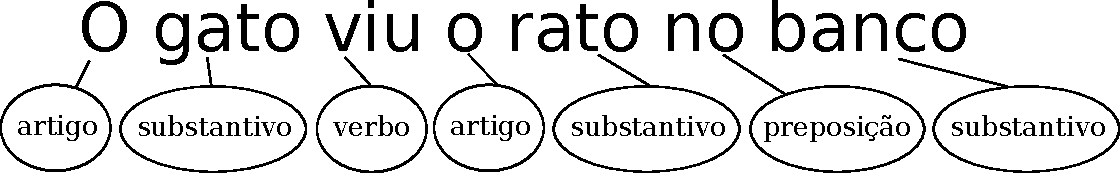
\includegraphics[scale=0.5]{img/exemploclassificacao.pdf}
    \end{center}
    % \caption{Exemplo de classificação gramatical}\label{fig:exemploclassificacao}
  \end{figure}

\end{frame}


\begin{frame}[fragile]
  \frametitle{O problema}

  

 \begin{itemize}
      \item Linguagens naturais são ambíguas 
      \item Estratégia trivial não é eficaz
      \item Necessário analisar o contexto
      \item Aprendizado de máquina
    \end{itemize}

  
    \begin{figure}[htb]
    \begin{center}
        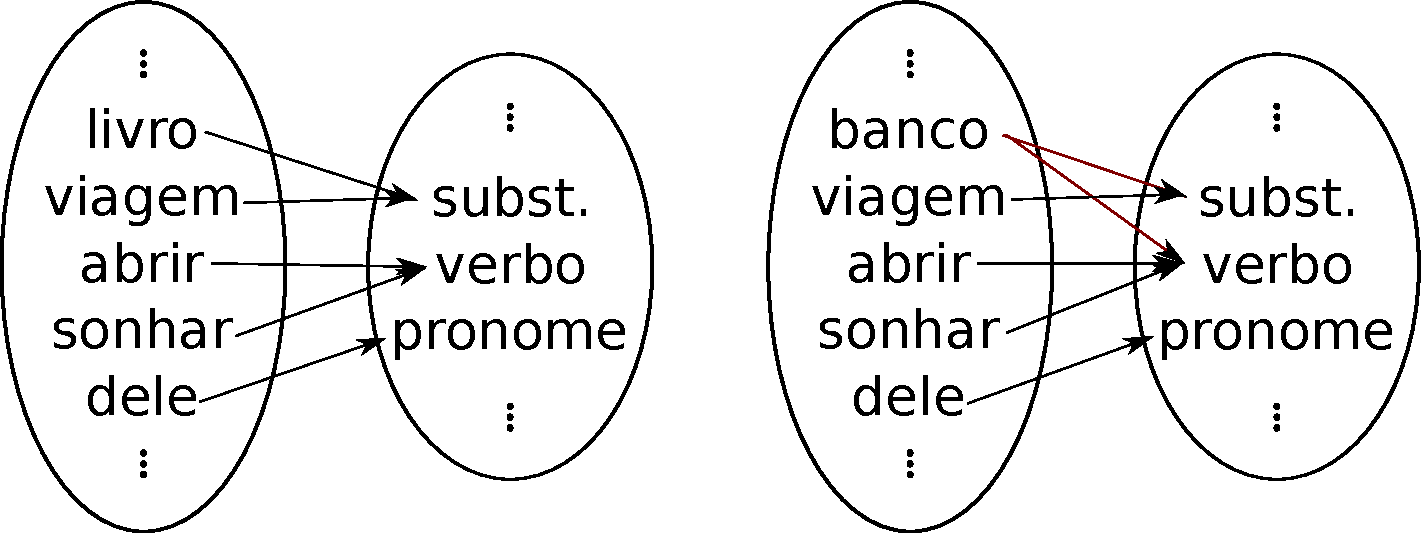
\includegraphics[scale=0.35]{img/funcoes.pdf}
    \end{center}
    % \caption{Função sobrejetora Vs. Função multivalorada}\label{fig:funcoes}
  \end{figure}

\end{frame}



\begin{frame}[fragile]
  \frametitle{Objetivos}


 \begin{itemize}
    \item Desenvolver novos modelos para POS Tagging
    \begin{itemize}
      \item[-] A princípio para o português brasileiro
    \end{itemize}
    \item[\ ] \ 
    \item Alcançar estado da arte
    \begin{itemize}
      \item[-] Combinar abordagens existentes
    \end{itemize}
     \item[\ ] \ 
    \item Analisar a acurácia
    \begin{itemize}
      \item[-] Palavras dentro do vocabulário
      \item[-] Palavras fora do vocabulário
      \item[-] Palavras ambíguas
      \item[-] Sentença
    \end{itemize}
  \end{itemize}

\end{frame}



\begin{frame}
  \frametitle{Roteiro}
  % \setbeamertemplate{section in toc}[mine]
  % \tableofcontents[hideallsubsections]


  \begin{itemize}

  % \vspace{-1em}

    
    \item[\color{gray}{$\bullet$}] \textcolor{gray}{Introdução}
    % \begin{itemize}
    %   \item[\ ] \textit{Part-of-speech} (POS) Tagging 
    %   \item[\ ] O problema
    %   \item[\ ] Objetivos
    % \end{itemize}
    
    
    \item Fundamentação
    \begin{itemize}
      \item[\ ] Aprendizado de máquina
      \item[\ ] Córpus
      \item[\ ] Representação de palavras
      \item[\ ] Redes neurais
      \item[\ ] Aprendizagem profunda
    \end{itemize}


    \color{gray}
    \item[\color{gray}{$\bullet$}] Trabalhos relacionados

    \item[\color{gray}{$\bullet$}] Modelo neural recursivo
    % \begin{itemize}
    %   \item[\ ] Pré-processamento
    %   \item[\ ] Arquitetura
    %   \item[\ ] Treinamento
    %   \item[\ ] Predição
    % \end{itemize}

    \item[\color{gray}{$\bullet$}] Modelo neural recorrente bidirecional
    % \begin{itemize}
    %   \item[\ ] Pré-processamento
    %   \item[\ ] Arquitetura
    %   \item[\ ] Treinamento
    %   \item[\ ] Predição
    % \end{itemize}

    \item[\color{gray}{$\bullet$}] Testes e resultados
    % \begin{itemize}
    %   \item[\ ] Ambiente de teste
    %   \item[\ ] Pré-processamento
    %   \item[\ ] Hiperparâmetros
    %   \item[\ ] Resultados
    %   \item[\ ] Comparação com trabalhos relacionados
    % \end{itemize}

    \item[\color{gray}{$\bullet$}] Considerações finais
    % \begin{itemize}
    %   \item[\ ] Conclusão
    %   \item[\ ] Trabalhos futuros
    % \end{itemize}

  \end{itemize}

\end{frame}


\section{Fundamentação}

\begin{frame}[fragile]
  \frametitle{Aprendizado de máquina}

  \only<1>{

    \begin{itemize}
      \item Aprendizado supervisionado
      \begin{itemize}
        \item[-] Regressão
        \item[-] Classificação  
      \end{itemize}
      \item Aprendizado não supervisionado
    \end{itemize}

    \begin{figure}[htb]
    \begin{center}
        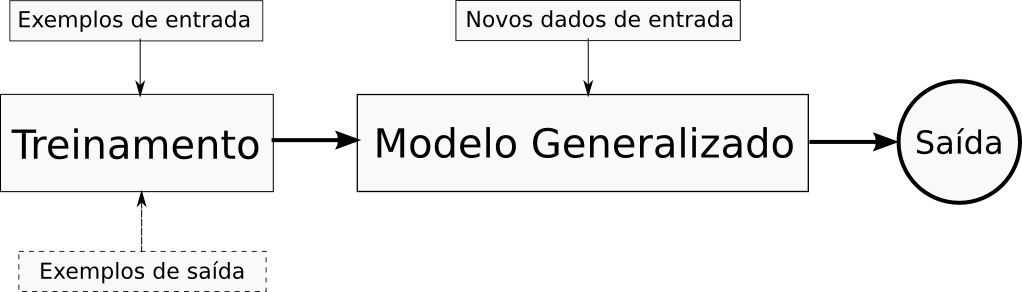
\includegraphics[scale=0.38]{img/passoapasso.png}
     % \caption{Matriz de coocorrência para criação de palavras vetorizadas} \label{fig:matrizdecoocorrencia}
    \end{center}
    \end{figure}

    \begin{equation}
    h_\theta(x) = \theta_0 + \theta_1f(x_1) + \theta_2 f(x_2) + ... + \theta_n f(x_n) \nonumber
    \end{equation}

  }


  \only<2>{

     \begin{itemize}
      \item Aprendizado supervisionado
      \begin{itemize}
        \item[-] \textbf{Regressão}
        \item[-] \textbf{Classificação}
      \end{itemize}
      \item Aprendizado não supervisionado
    \end{itemize}

  \begin{columns}[onlytextwidth]
    \column{0.5\textwidth}
    \begin{figure}[htb]
    \begin{center}
        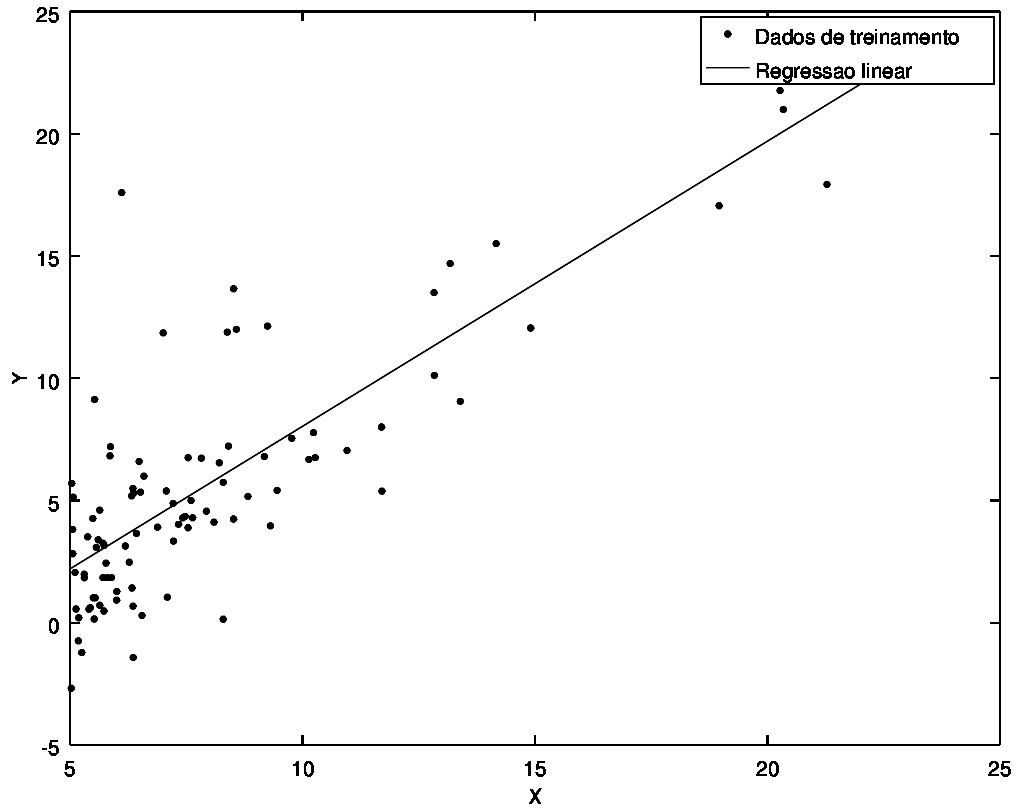
\includegraphics[width=\textwidth]{img/regressao2x.png}
    \end{center}
    \end{figure}  
    

    \column{0.5\textwidth}
    \begin{figure}[htb]
    \begin{center}
        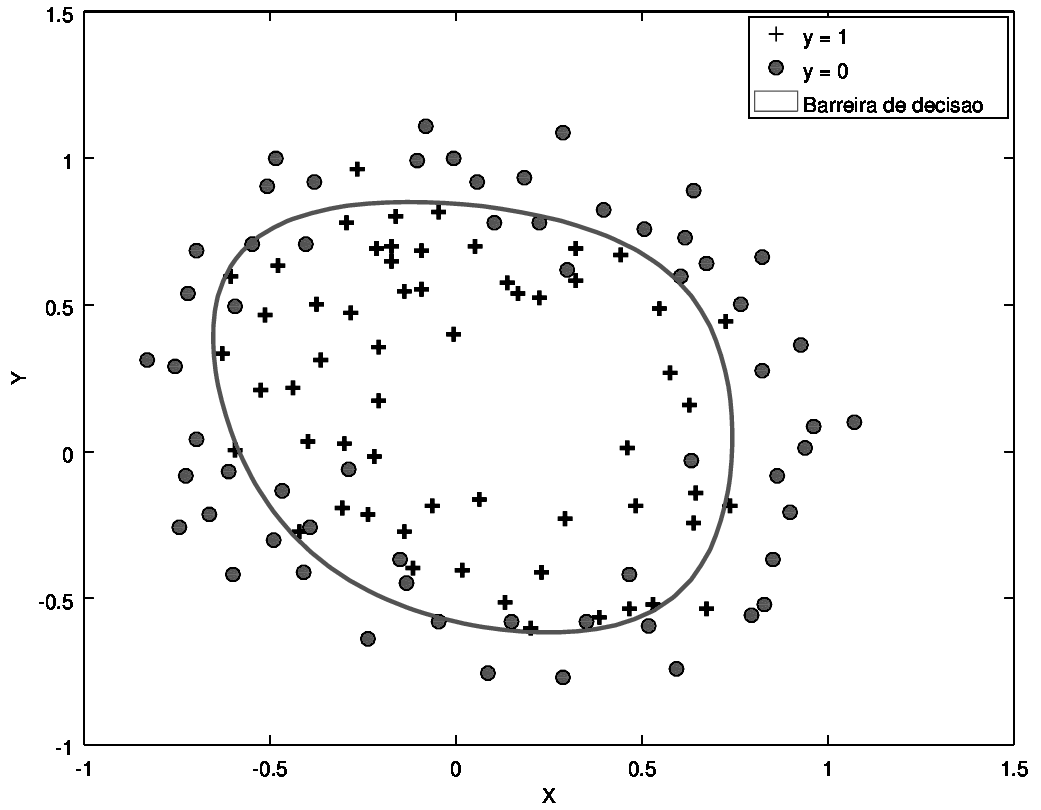
\includegraphics[width=\textwidth]{img/classificacao2x.png}
    \end{center}
    \end{figure}  


  \end{columns}

    

  }


  

\end{frame}



\begin{frame}[fragile]
  \frametitle{Córpus}

  \begin{itemize}
    \item Coleções de textos agrupados
    \item Anotação gramatical manual
    \item \textit{Córpus} para o português brasileiro:\\ \

    \begin{table}[!htb]
    \footnotesize
    \centering
    \begin{tabular}{lccc}
      \toprule
      \textbf{Córpus} & \textbf{Sentenças}  & \textbf{Palavras}  & \textbf{Classes gramaticais}  \\
      \midrule
      Mac-Morpho original & 53,374 & 1,221,465 & 41  \\
      Mac-Morpho revisado\footnotemark & 49,932 & 945,958   & 26  \\
      Tycho Brahe         & 55,932 & 1,541,654 & 265 \\
      \bottomrule
    \end{tabular}
    % \caption{Dados dos \textit{córpus}} \label{tab:dadoscorpus}
    \end{table}

  \item[\ ] \ 
  \item Por que não combiná-los?
  \item[\ ] \ 
  \end{itemize}


{\scriptsize 1. Revisado por: \citeonline{fonseca2015evaluating}.}

\end{frame}



\begin{frame}[fragile]
  \frametitle{Representação de palavras}

  \begin{itemize}

    \item Vetores reais valorados em um espaço multidimensional (\textit{word embeddings})
    
    \item[\ ] \ 

    \item Mais desempenho de aplicações em PLN e menos engenharia de \textit{features}

    \item[\ ] \ 

    \item Conseguem capturar informações sintáticas e semânticas

    \item[\ ] \ 

    \item Geradas de maneiras diferentes dependendo da técnica utilizada
    \begin{itemize}
      \item[-] Word2Vec, Wang2Vec, GloVe, etc.
    \end{itemize}


    \item[\ ] \ 

    \item Palavras fora do vocabulário de treinamento podem ter seu próprio vetor


  \end{itemize}
  


\end{frame}



\begin{frame}[fragile]
  \frametitle{Representação de palavras}

   \begin{itemize}
    \item[\ ] \
    \item Palavras similares estão próximas
     
  \end{itemize}

  \begin{figure}[htb]
    \begin{center}
        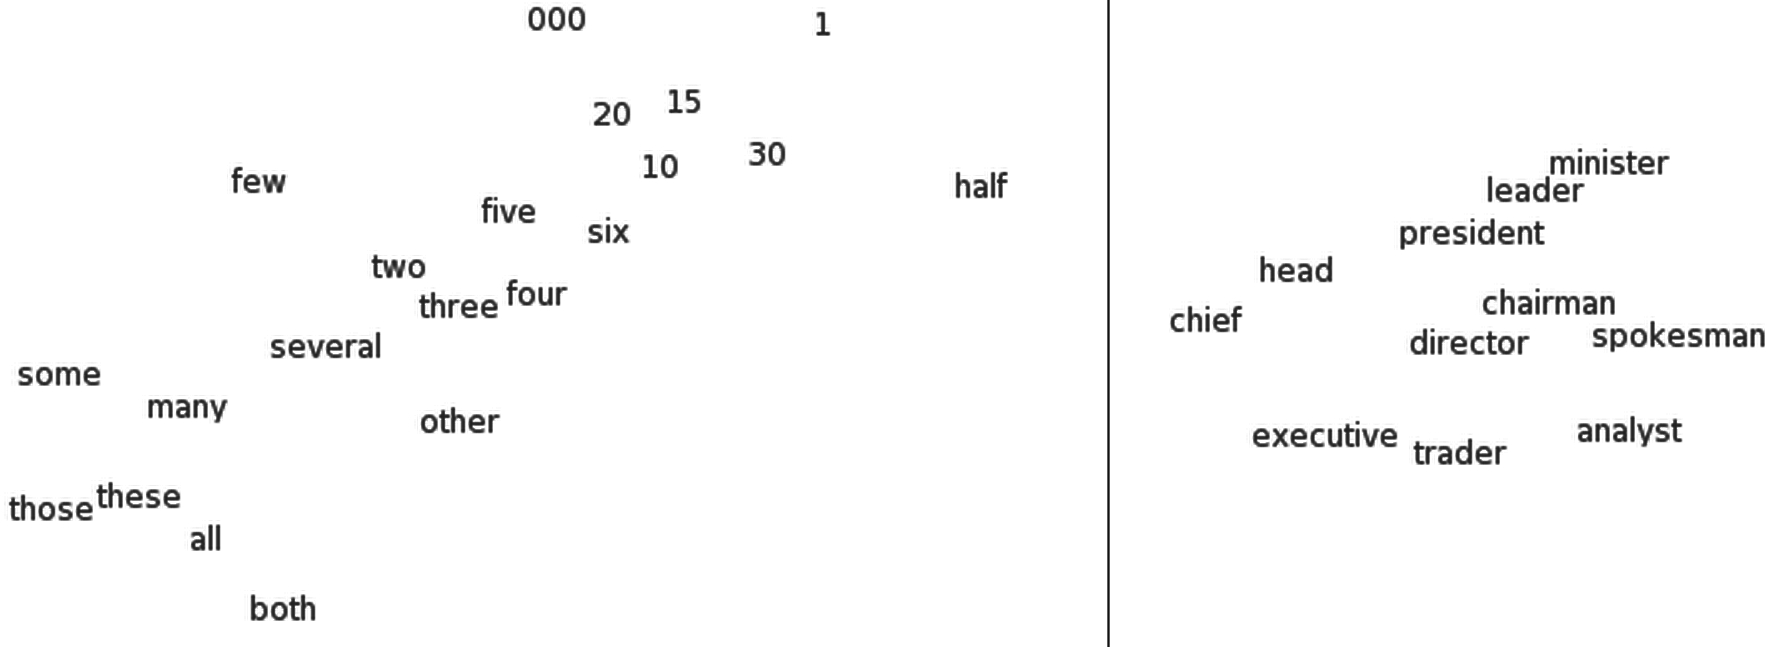
\includegraphics[scale=0.18]{img/Turian-WordTSNE}
    \end{center}
    \caption{Imagem criada pelo t-SNE\\Fonte: \citeonline{turian2010word}}

  \end{figure}
\end{frame}





\begin{frame}[fragile]
  \frametitle{Redes neurais}

  \begin{columns}[onlytextwidth]
    \column{0.5\textwidth}
      
      \begin{itemize}
        \item Simulação do cérebro humano
        \item[\ ] \ 
        \item Unidades de ativação: $a_i^{(j)}$
        \item[\ ] \ 
        \item Pesos: $\theta^{(j)}$
        \item[\ ] \ 
        \item Função de ativação: $g(\cdot)$
        \item[\ ] \ 
        \item $a^{(j+1)} = g(\theta^{(j)}a^{(j)})$
        \item[\ ] \ 
        \item \textit{Forward propagation} e \textit{Backpropagation}
      \end{itemize}


    \column{0.5\textwidth}

    \only<1>{
        \begin{figure}[!htb]
        \begin{center}
        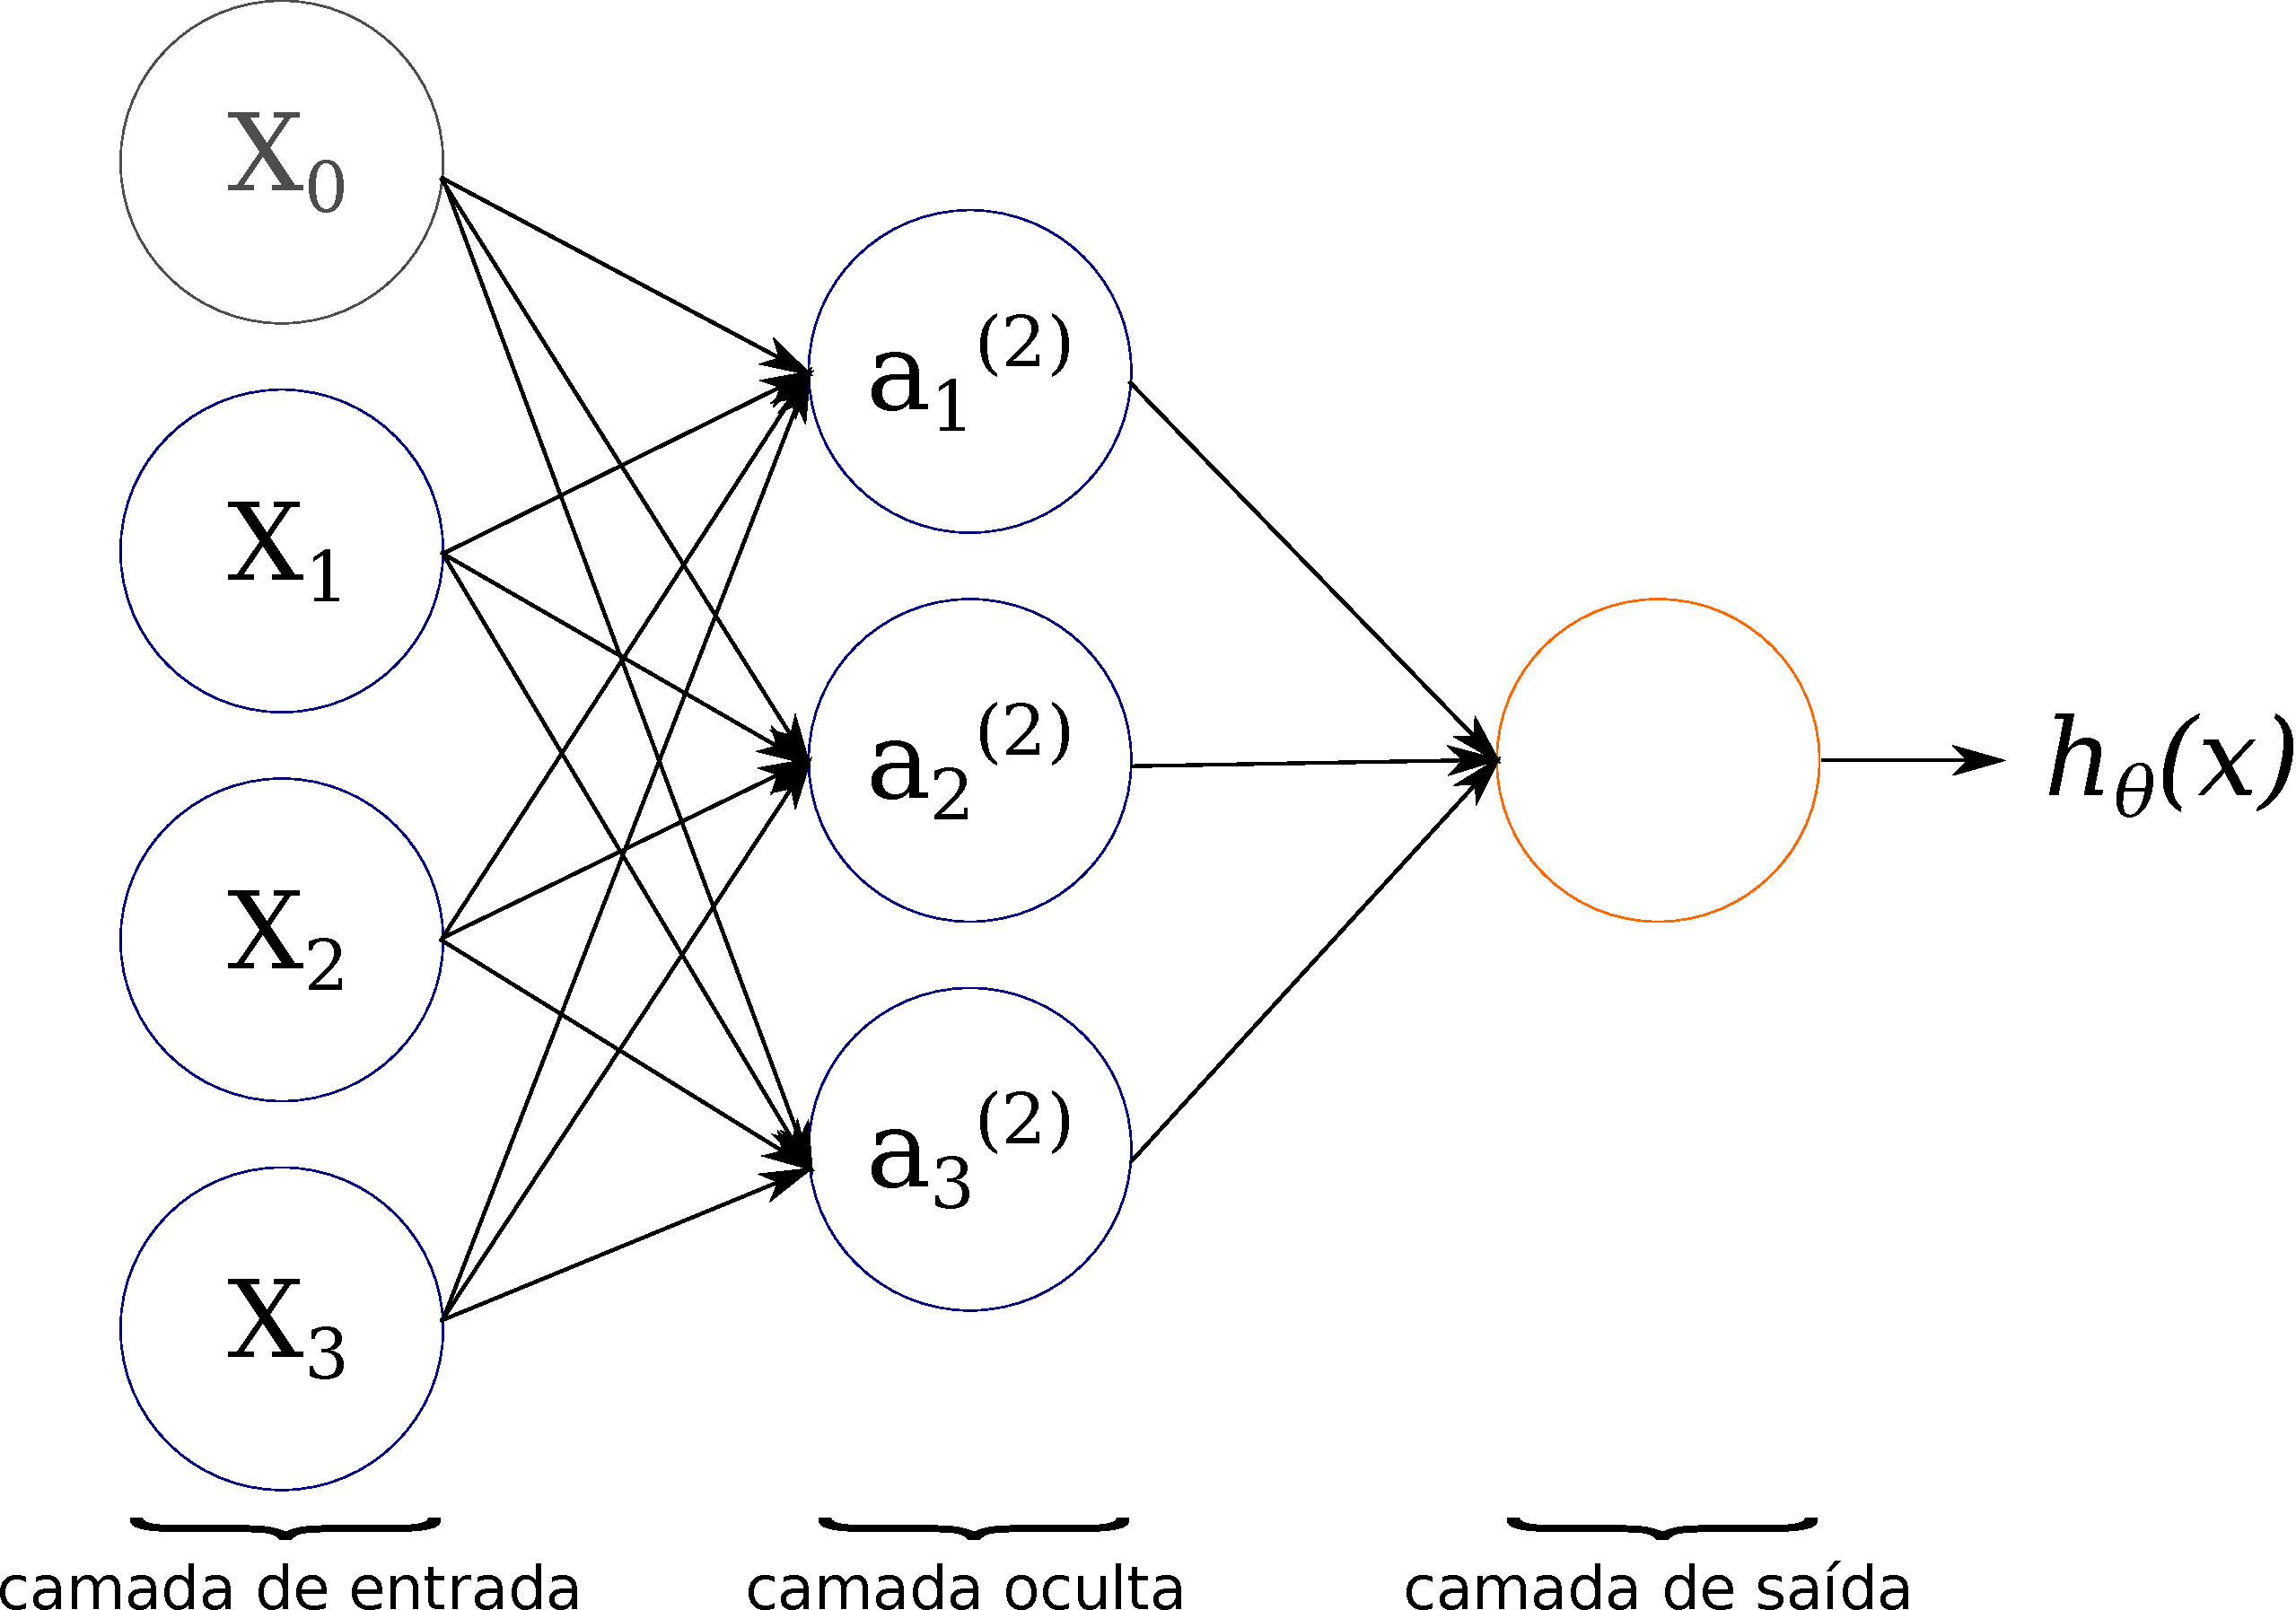
\includegraphics[width=\textwidth]{img/redeneuraloculta2.pdf}
        \end{center}
        \end{figure}
    }

    \only<2>{
      
       \begin{figure}[!htb]
        \begin{center}
        \begin{tikzpicture}
        \begin{axis}[
            width=1.0\textwidth,
            scaled ticks=false,
            log ticks with fixed point,
            ymin=0,ymax=1,xmin=-10,xmax=10,domain=-10:10,
            log basis y = 10,
            title={Função sigmoide},
            xlabel=x,
            ylabel=y,
            legend style={draw=none},
            samples=200,
          ]
          \addplot[blue] { 1 / (1 + pow(e, -x))};
        \end{axis}
        \end{tikzpicture}
        \end{center}
        \end{figure}
      }

  \end{columns}

\end{frame}


\begin{frame}[fragile]
  \frametitle{Aprendizagem profunda}

   \begin{itemize}
    \item Muitas tranformações não lineares

    \item Extração automática de \textit{features}
    
    \item Redes neurais profundas

    \begin{itemize}
      \item[-] Redes neurais convolucionais
      \item[-] Redes neurais recursivas
      \item[-] Redes neurais recorrentes
        \begin{itemize}
          \item[\ ] \textit{Long Short Term Memory} (LSTM)
          \item[\ ] \textit{Gated Recurrent Unit} (GRU) 
          \item[\ ] Bidirecional
        \end{itemize}
    \end{itemize}

  \end{itemize}

  \begin{figure}[b]
    \begin{center}
        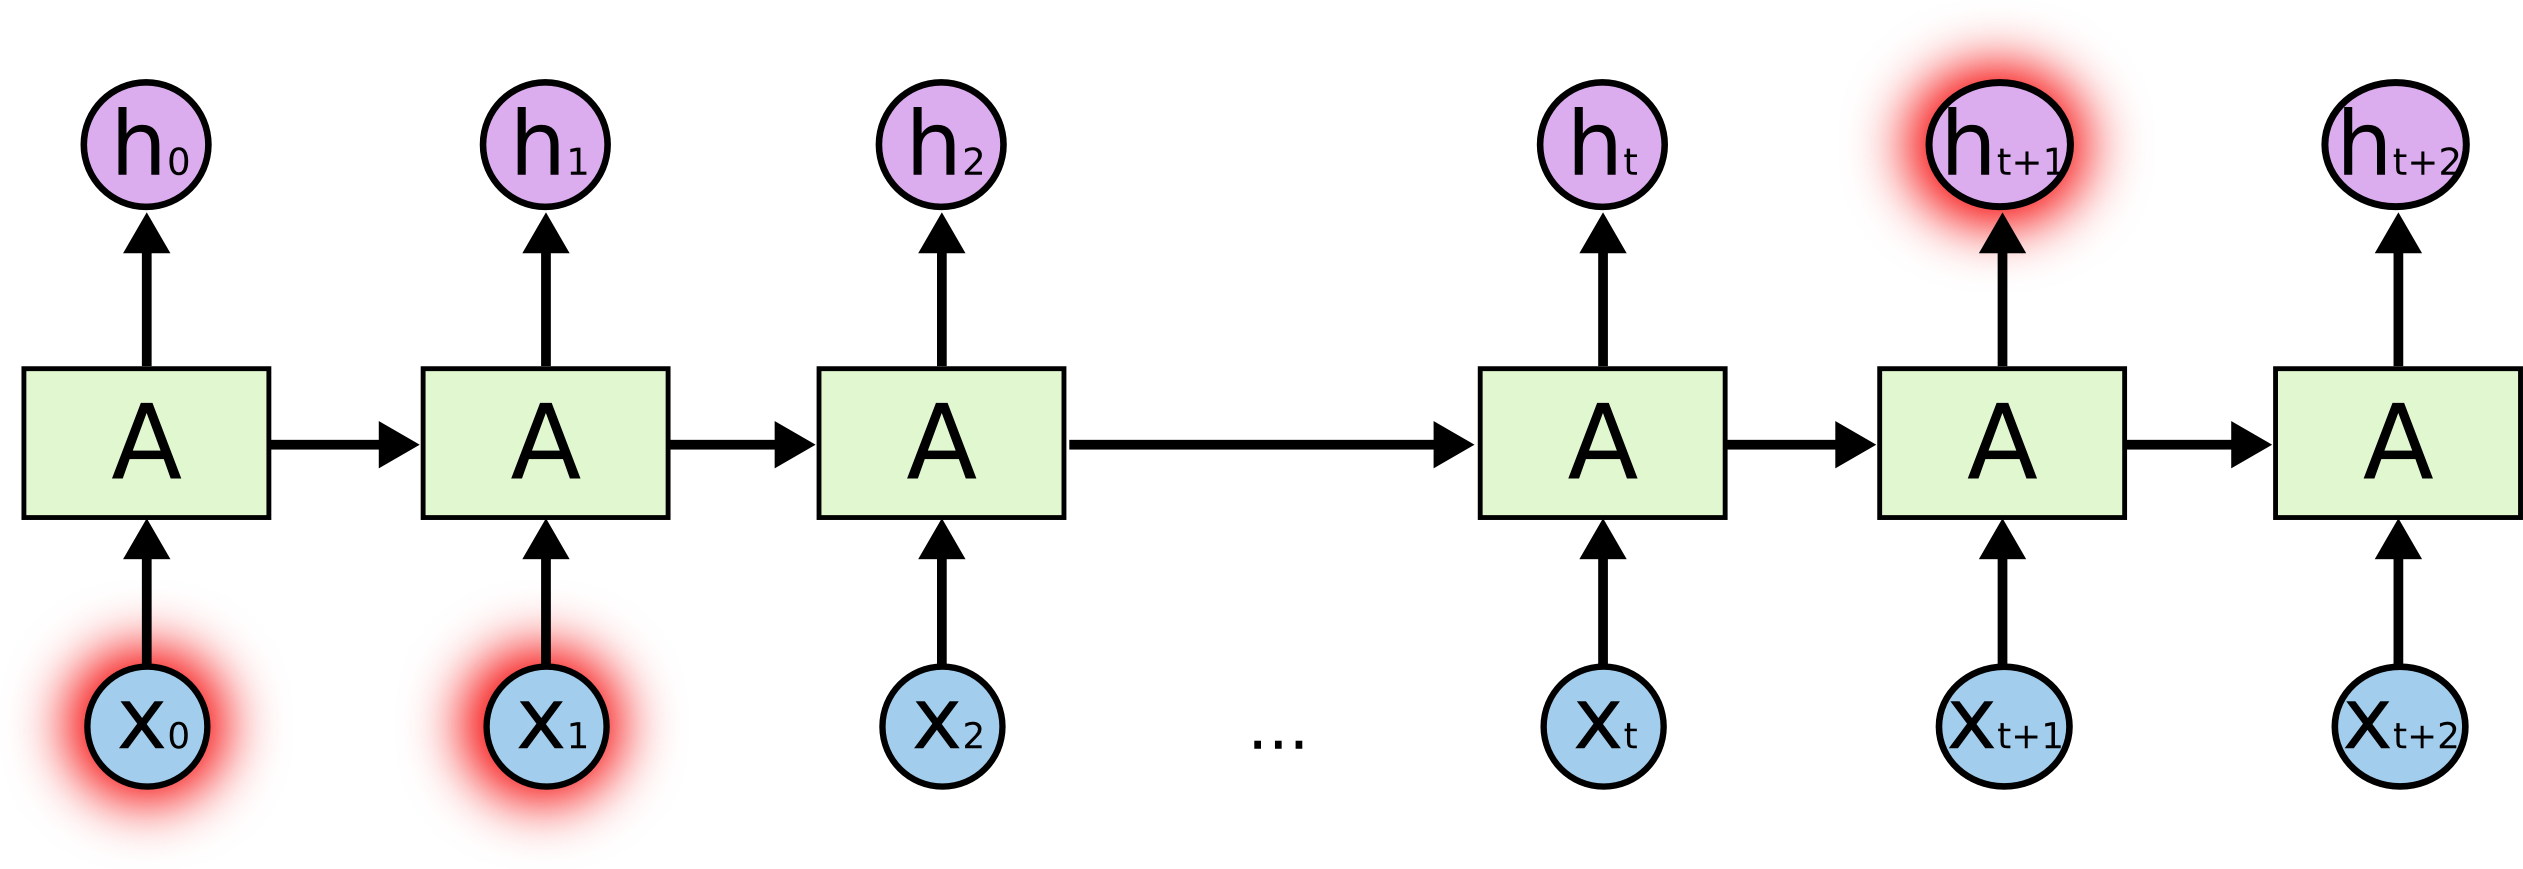
\includegraphics[scale=0.25]{img/rnn_longtermdependencies.png}
    \end{center}
    \caption{Exemplo de rede neural recorrente com longa dependência\\Fonte: \citeonline{lstmnet}}

  \end{figure}
  

\end{frame}




\begin{frame}
  \frametitle{Roteiro}
  % \setbeamertemplate{section in toc}[mine]
  % \tableofcontents[hideallsubsections]


  \begin{itemize}

  % \vspace{-1em}

    
    \item[\color{gray}{$\bullet$}] \textcolor{gray}{Introdução}
    % \begin{itemize}
    %   \item[\ ] \textit{Part-of-speech} (POS) Tagging 
    %   \item[\ ] O problema
    %   \item[\ ] Objetivos
    % \end{itemize}
    
    
    \item[\color{gray}{$\bullet$}] \textcolor{gray}{Fundamentação}
    % \begin{itemize}
    %   \item[\ ] Aprendizado de máquina
    %   \item[\ ] Córpus
    %   \item[\ ] Representação de palavras
    %   \item[\ ] Redes neurais
    %   \item[\ ] Aprendizagem profunda
    % \end{itemize}


    
    \item Trabalhos relacionados

    \color{gray}
    \item[\color{gray}{$\bullet$}] Modelo neural recursivo
    % \begin{itemize}
    %   \item[\ ] Pré-processamento
    %   \item[\ ] Arquitetura
    %   \item[\ ] Treinamento
    %   \item[\ ] Predição
    % \end{itemize}

    \item[\color{gray}{$\bullet$}] Modelo neural recorrente bidirecional
    % \begin{itemize}
    %   \item[\ ] Pré-processamento
    %   \item[\ ] Arquitetura
    %   \item[\ ] Treinamento
    %   \item[\ ] Predição
    % \end{itemize}

    \item[\color{gray}{$\bullet$}] Testes e resultados
    % \begin{itemize}
    %   \item[\ ] Ambiente de teste
    %   \item[\ ] Pré-processamento
    %   \item[\ ] Hiperparâmetros
    %   \item[\ ] Resultados
    %   \item[\ ] Comparação com trabalhos relacionados
    % \end{itemize}

    \item[\color{gray}{$\bullet$}] Considerações finais
    % \begin{itemize}
    %   \item[\ ] Conclusão
    %   \item[\ ] Trabalhos futuros
    % \end{itemize}

  \end{itemize}

\end{frame}



\section{Trabalhos relacionados}

\begin{frame}[fragile]
  \frametitle{Trabalhos relacionados}

  \begin{itemize}

  \item Escopo do português brasileiro

  \end{itemize}

  \hspace*{0cm}\makebox[\linewidth][c]{
  \scriptsize
    \begin{tabular}{llll}
      \toprule
      \textbf{Autores} & \textbf{Modelo}  & \textbf{Rep. palavras}  & \textbf{Córpus} \\
      \midrule
      \citeonline{kepler2010variable}     & VLMC & Seq. de carac.      & Tycho Brahe \\
      \hline
      \citeonline{dos2014training}        & RNs  & Vet. de pal. e carac.  & \begin{tabular}[l]{@{}l@{}}Tycho Brahe; \\ Mac-Morpho v1, v2\end{tabular} \\
      \hline
      \citeonline{fonseca2015evaluating}  & RNs                    & Vet. de palavras & \begin{tabular}[l]{@{}l@{}}Tycho Brahe; \\ Mac-Morpho v1, v2, v3\end{tabular}  \\
      \hline
      Este trabalho                       & RNs recur. e recor.    & Vet. de palavras &  \begin{tabular}[l]{@{}l@{}}Tycho Brahe; \\ Mac-Morpho v1, v3\end{tabular} \\
      \bottomrule
    \end{tabular}
  }

  % \item[\ ] \adjustbox{max height=\dimexpr\textheight-5.5cm\relax,max width=\textwidth}{
  % \begin{tabular}{llllc}
  %   \toprule
  %   \textbf{Autores} & \textbf{Modelo}  & \textbf{Rep. palavras}  & \textbf{Córpus} & \textbf{Acurácia} \\
  %   \midrule
  %   \citeonline{kepler2005etiquetador} & VLMC & Seq. de carac. & Tycho Brahe & 95,51\% \\
  %   \citeonline{dos2014training} & Redes neurais profundas  & Vetores & Tycho Brahe; Mac-Morpho & 97,47\% \\
  %   \citeonline{fonseca2015evaluating} & Redes neurais & Vetores & Tycho Brahe; Mac-Morpho & 97,57\% \\
  %   Este trabalho & Redes neurais recursivas & Vetores & Tycho Brahe; Mac-Morpho & - \\
  %   \bottomrule
  % \end{tabular}
  % }

  \ 

  \begin{itemize}
    \item[\ ] \ 
    \item Estado da arte
  \end{itemize}
  \vspace{-0.3cm}
  \begin{table}[!htb]
  \scriptsize
  \begin{center}
  \begin{tabular}{lcc}
    \toprule
    \textbf{Córpus} & \textbf{Autores} & \textbf{Acurácia}  \\
    \midrule
    Mac-Morpho v1 (original) & \citeonline{fonseca2015evaluating} & 97.57\% \\
    Mac-Morpho v3 (revisado) & \citeonline{fonseca2015evaluating} & 97.33\% \\
    Tycho Brahe              & \citeonline{dos2014training} & 97.17\% \\
    \bottomrule
  \end{tabular}
  \end{center}
  \end{table}
 

\end{frame}






\begin{frame}
  \frametitle{Roteiro}
  % \setbeamertemplate{section in toc}[mine]
  % \tableofcontents[hideallsubsections]


  \begin{itemize}

  % \vspace{-1em}

    
    \item[\color{gray}{$\bullet$}] \textcolor{gray}{Introdução}
    % \begin{itemize}
    %   \item[\ ] \textit{Part-of-speech} (POS) Tagging 
    %   \item[\ ] O problema
    %   \item[\ ] Objetivos
    % \end{itemize}
    
    
    \item[\color{gray}{$\bullet$}] \textcolor{gray}{Fundamentação}
    % \begin{itemize}
    %   \item[\ ] Aprendizado de máquina
    %   \item[\ ] Córpus
    %   \item[\ ] Representação de palavras
    %   \item[\ ] Redes neurais
    %   \item[\ ] Aprendizagem profunda
    % \end{itemize}


    
    \item[\color{gray}{$\bullet$}] \textcolor{gray}{Trabalhos relacionados}

    
    \item Modelo neural recursivo
    \begin{itemize}
      \item[\ ] Pré-processamento
      \item[\ ] Arquitetura
      \item[\ ] Treinamento
      \item[\ ] Predição
    \end{itemize}

    \color{gray}
    \item[\color{gray}{$\bullet$}] Modelo neural recorrente bidirecional
    % \begin{itemize}
    %   \item[\ ] Pré-processamento
    %   \item[\ ] Arquitetura
    %   \item[\ ] Treinamento
    %   \item[\ ] Predição
    % \end{itemize}

    \item[\color{gray}{$\bullet$}] Testes e resultados
    % \begin{itemize}
    %   \item[\ ] Ambiente de teste
    %   \item[\ ] Pré-processamento
    %   \item[\ ] Hiperparâmetros
    %   \item[\ ] Resultados
    %   \item[\ ] Comparação com trabalhos relacionados
    % \end{itemize}

    \item[\color{gray}{$\bullet$}] Considerações finais
    % \begin{itemize}
    %   \item[\ ] Conclusão
    %   \item[\ ] Trabalhos futuros
    % \end{itemize}

  \end{itemize}

\end{frame}


\section{Modelo neural recursivo}


\begin{frame}[fragile]
\frametitle{Pré-processamento}


  \begin{itemize}
    \item Janela de palavras com tamanho $t$:
  \end{itemize}

  \begin{equation} \nonumber
    V_n = \big\{ \imath(w_{n - \lfloor t/2 \rfloor}), ..., \imath(w_n), ..., \imath(w_{n + \lfloor t/2 \rfloor}) \big\}
  \end{equation}

  \begin{itemize}
    \item Janela de etiquetas com o mesmo tamanho que a janela de palavras
  \end{itemize}

  \begin{itemize}
    \item \texttt{<mask>}: Para as extremidades das janelas
    \item \texttt{<unknown>}: Para palavras raras ou desconhecidas
    \item \texttt{<padding\_prefix>}: Para completar o vetor de prefixos
    \item \texttt{<padding\_suffix>}: Para completar o vetor de sufixos
  \end{itemize}

\end{frame}



\begin{frame}[fragile]
\frametitle{Arquitetura}
  
  % \vspace{-0.75em}
  

  \begin{figure}
      \begin{center}
        \hspace*{-2em}
        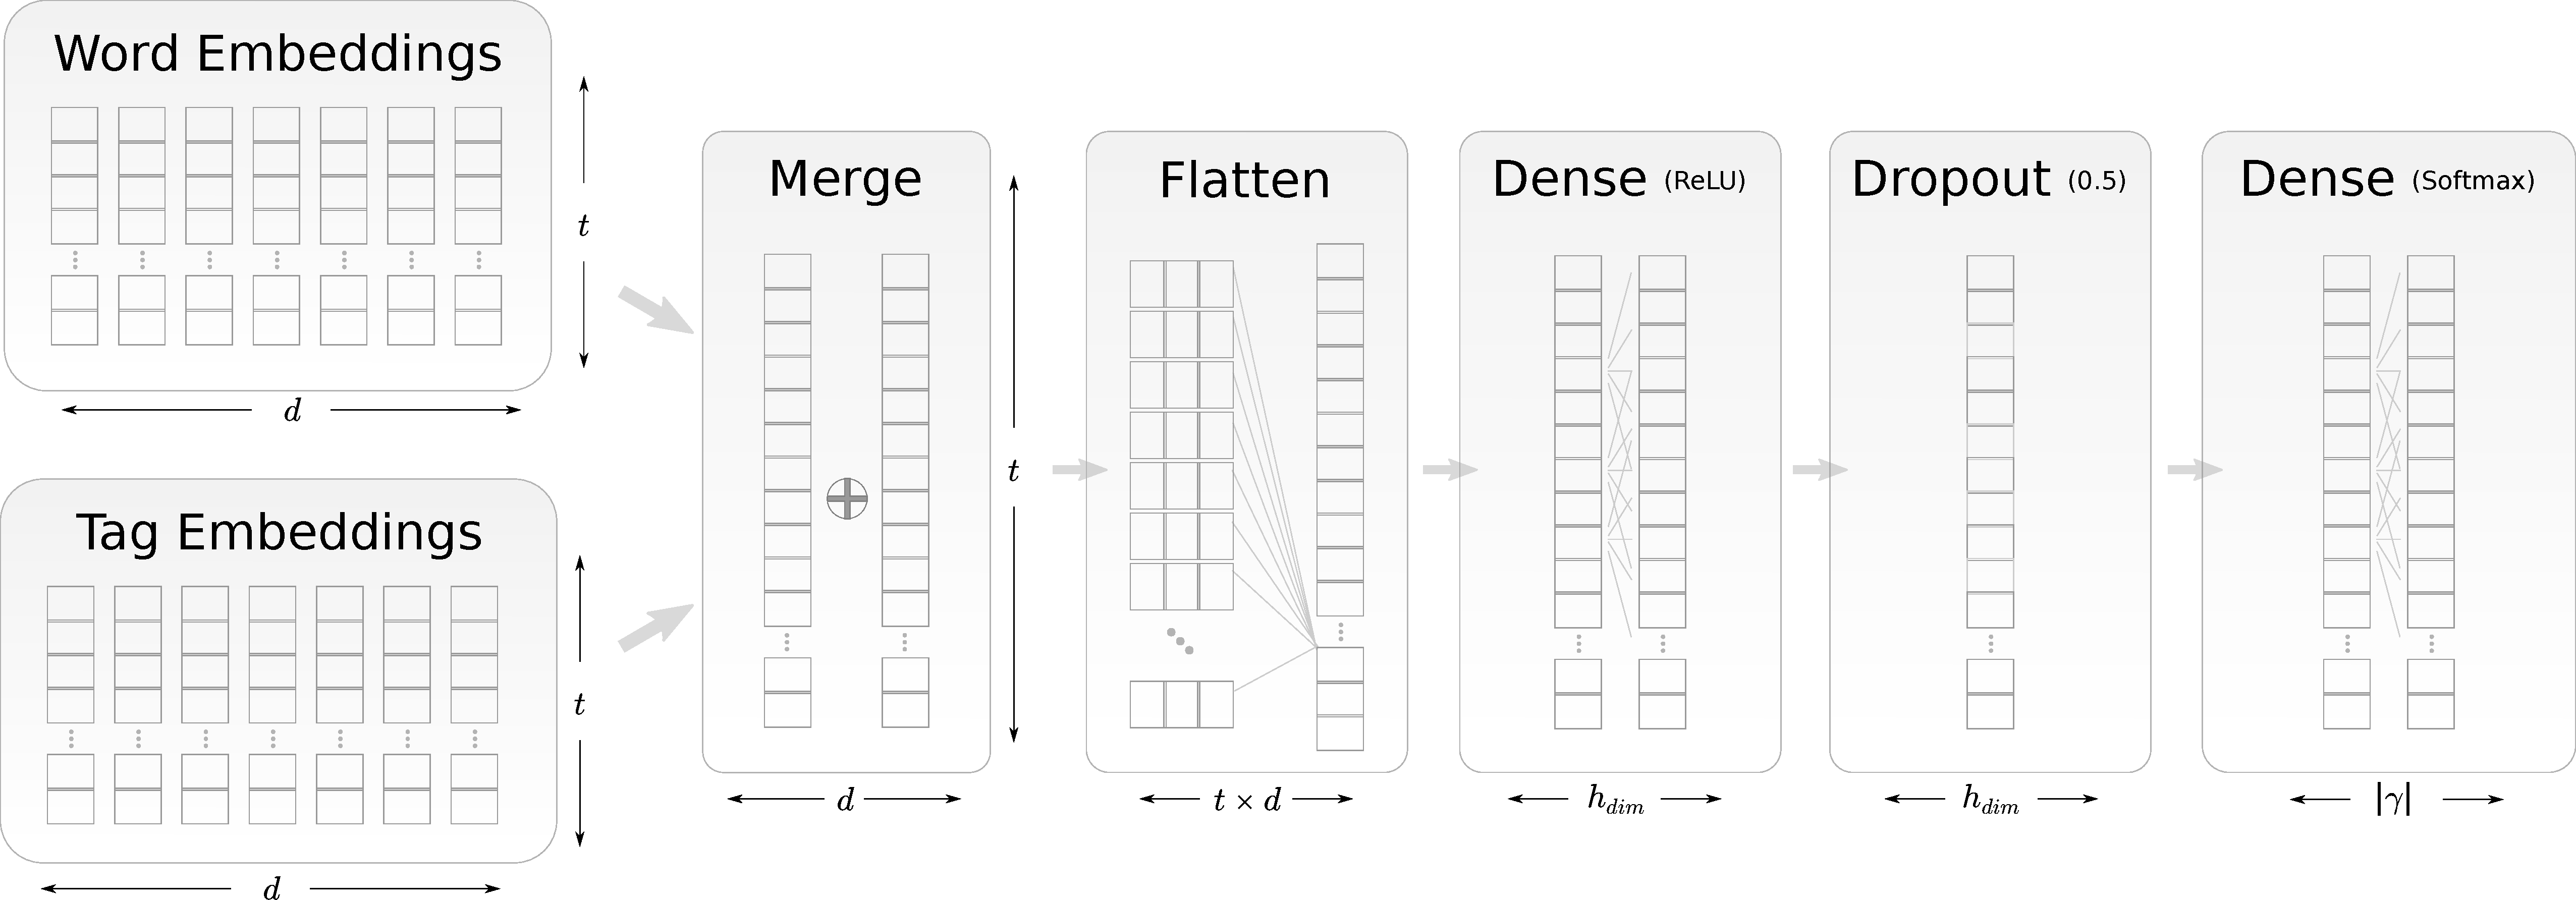
\includegraphics[scale=0.14]{img/recursive_model_horizontal.pdf}
      \end{center}
  \end{figure}

\begin{equation} \nonumber
ReLU(x) = max(0, x)
\end{equation}

\begin{equation}  \nonumber
softmax(x) = \frac{e^{x_j}}{\sum_{k=1}^{n} e^{x_k}}, \quad \mbox{para } j = 1, ..., n
\end{equation}


\end{frame}



\begin{frame}[fragile]
\frametitle{Treinamento}
  
  \begin{itemize}

    \item Guiado por palavras mais fáceis \cite{shen2007guided}


  \end{itemize}

  \begin{table}[!htb]
  \scriptsize
  \begin{center}
  \begin{tabular}{c|c|c|c}
    \toprule
    Palavra/Etiqueta & substantivo & adjetivo & verbo \\
    \midrule
    Computação & 0.6 & 0.2 & 0.2 \\
    \midrule
    é          & 0.7 & 0.2 & 0.1 \\
    \midrule
    um         & 0.1 & 0.6 & 0.3 \\
    \midrule
    curso      & \textbf{0.8} & 0.1 & 0.1 \\
    \midrule
    legal      & 0.4 & 0.4 & 0.2 \\
    \midrule
    !          & 0.5 & 0.4 & 0.1 \\
    \bottomrule
  \end{tabular}
  \end{center}
  \end{table}

  \begin{itemize}
  \item[\ ] $mp(M) = \argmax\limits_{i \not \in Q}\Big(\max\limits_{0 \leq j < |\gamma|}(M_{i,j})\Big)$
  \item[\ ] \   
  \item[\ ]  $J_c[mp(M)-\lfloor t/2 \rfloor:mp(M)+\lfloor t/2 \rfloor][I_t] = c_{mp(M)}$
  \end{itemize}

\end{frame}



\begin{frame}[fragile]
\frametitle{Predição}
  
  % \begin{figure}
  %     \begin{center}
  %       \hspace*{-2em}
  %       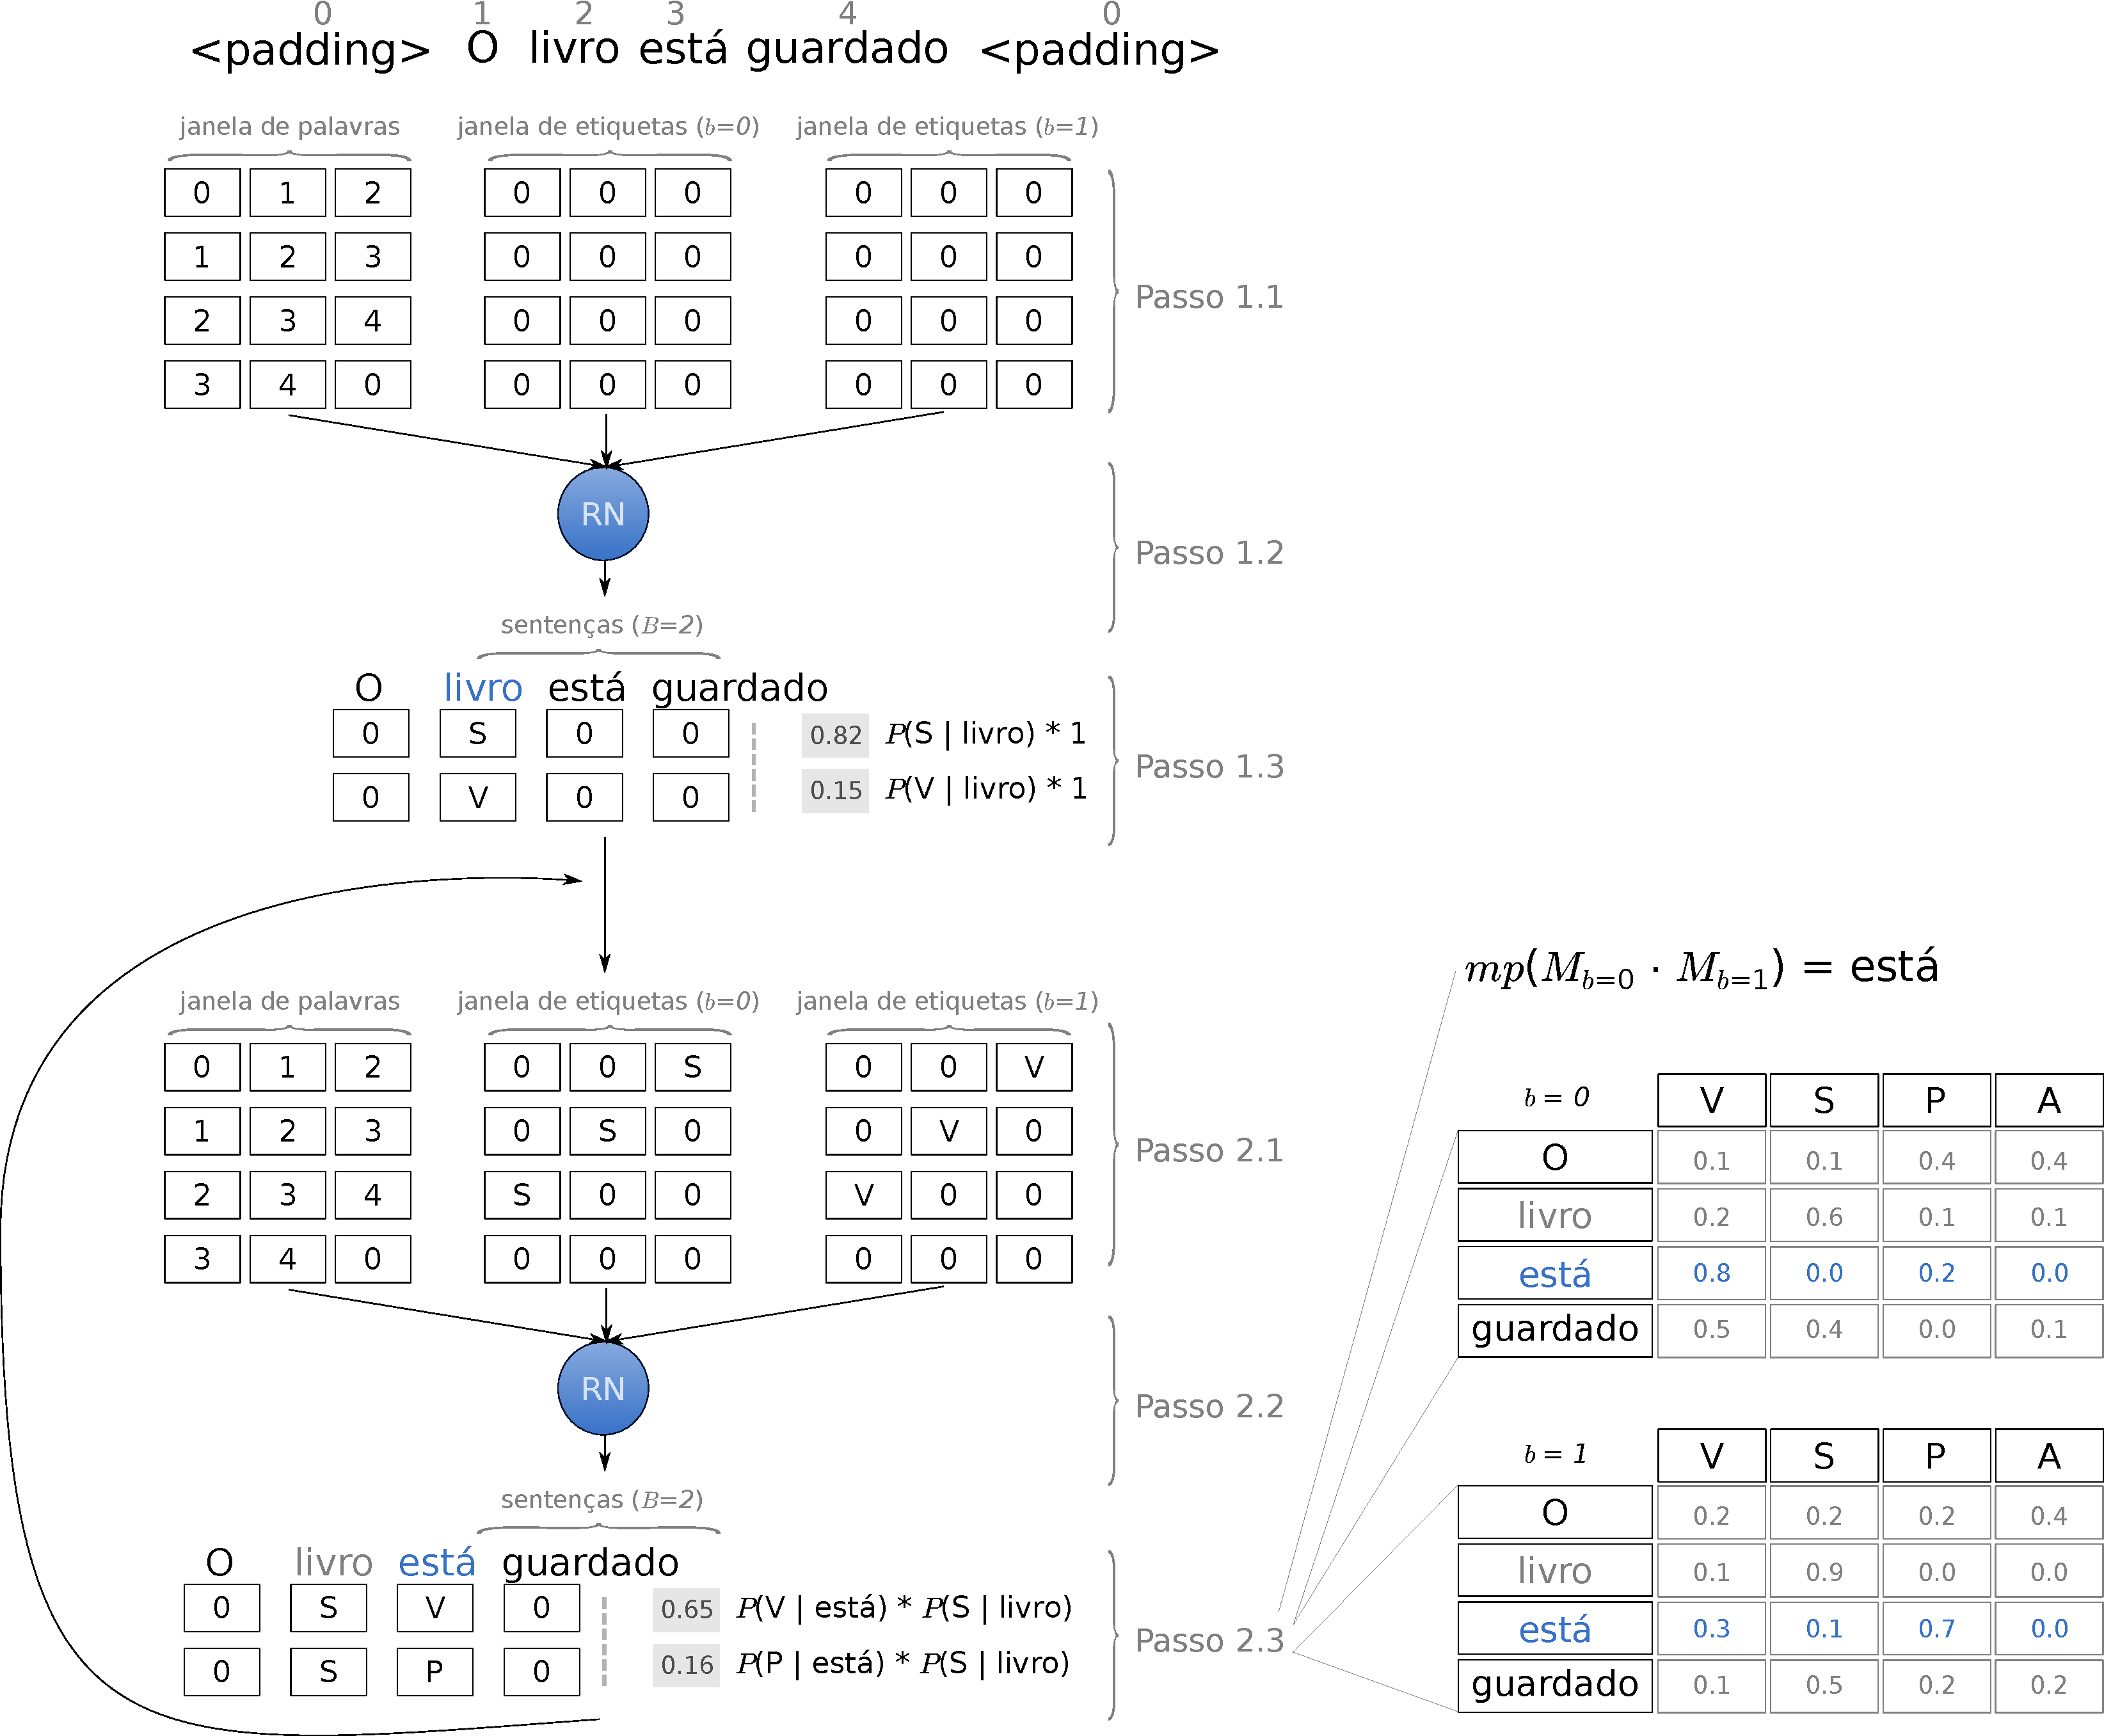
\includegraphics[scale=0.17]{img/algoritmodepredicao.pdf}
  %     \end{center}
  % \end{figure}
  


  \begin{itemize}

    \item Semelhante ao algoritmo treinamento

    \item[\ ] \   

    \item \textit{Beam search} de tamanho $B$

    \item[\ ] \   

    \item $B$ sequências de etiquetas mais prováveis para a sentença

    \item[\ ] \   

    \item Dá para resumir nas seguintes etapas:

    \begin{enumerate}
      \item Inicialização (pré-processamento)
      \item Atualização da janela de etiquetas
      \item Predição na rede neural 
      \item Atualização das $B$ sentenças de acordo com a palavra mais provável
      \begin{itemize}
        \item[-] Levando em consideração a probabilidade da sentença e a probabilidade de emissão da etiqueta
      \end{itemize}
    \end{enumerate}

  \end{itemize}

\end{frame}






\begin{frame}
  \frametitle{Roteiro}
  % \setbeamertemplate{section in toc}[mine]
  % \tableofcontents[hideallsubsections]


  \begin{itemize}

  % \vspace{-1em}

    
    \item[\color{gray}{$\bullet$}] \textcolor{gray}{Introdução}
    % \begin{itemize}
    %   \item[\ ] \textit{Part-of-speech} (POS) Tagging 
    %   \item[\ ] O problema
    %   \item[\ ] Objetivos
    % \end{itemize}
    
    
    \item[\color{gray}{$\bullet$}] \textcolor{gray}{Fundamentação}
    % \begin{itemize}
    %   \item[\ ] Aprendizado de máquina
    %   \item[\ ] Córpus
    %   \item[\ ] Representação de palavras
    %   \item[\ ] Redes neurais
    %   \item[\ ] Aprendizagem profunda
    % \end{itemize}


    
    \item[\color{gray}{$\bullet$}] \textcolor{gray}{Trabalhos relacionados}

    
    \item[\color{gray}{$\bullet$}] \textcolor{gray}{Modelo neural recursivo}
    % \begin{itemize}
    %   \item[\ ] Pré-processamento
    %   \item[\ ] Arquitetura
    %   \item[\ ] Treinamento
    %   \item[\ ] Predição
    % \end{itemize}

    
    \item Modelo neural recorrente bidirecional
    \begin{itemize}
      \item[\ ] Pré-processamento
      \item[\ ] Arquitetura
      \item[\ ] Treinamento e Predição
    \end{itemize}


    \color{gray}
    \item[\color{gray}{$\bullet$}] Testes e resultados
    % \begin{itemize}
    %   \item[\ ] Ambiente de teste
    %   \item[\ ] Pré-processamento
    %   \item[\ ] Hiperparâmetros
    %   \item[\ ] Resultados
    %   \item[\ ] Comparação com trabalhos relacionados
    % \end{itemize}

    \item[\color{gray}{$\bullet$}] Considerações finais
    % \begin{itemize}
    %   \item[\ ] Conclusão
    %   \item[\ ] Trabalhos futuros
    % \end{itemize}

  \end{itemize}

\end{frame}


\section{Modelo neural recorrente bidirecional}

\begin{frame}[fragile]
\frametitle{Pré-processamento}


  \begin{itemize}
    \item Janela de palavras com tamanho $t$:
  \end{itemize}

  \begin{equation} \nonumber
    V_n = \big\{ \imath(w_{n - \lfloor t/2 \rfloor}), ..., \imath(w_n), ..., \imath(w_{n + \lfloor t/2 \rfloor}) \big\}
  \end{equation}

  \begin{itemize}
    \item \texttt{<mask>}: Para as extremidades das janelas
    \item \texttt{<unknown>}: Para palavras raras ou desconhecidas
    \item \texttt{<padding\_prefix>}: Para completar o vetor de prefixos
    \item \texttt{<padding\_suffix>}: Para completar o vetor de sufixos
  \end{itemize}

\end{frame}



\begin{frame}[fragile]
\frametitle{Arquitetura}
  
  % \vspace{-0.75em}
  

  \begin{figure}
      \begin{center}
        \hspace*{-2em}
        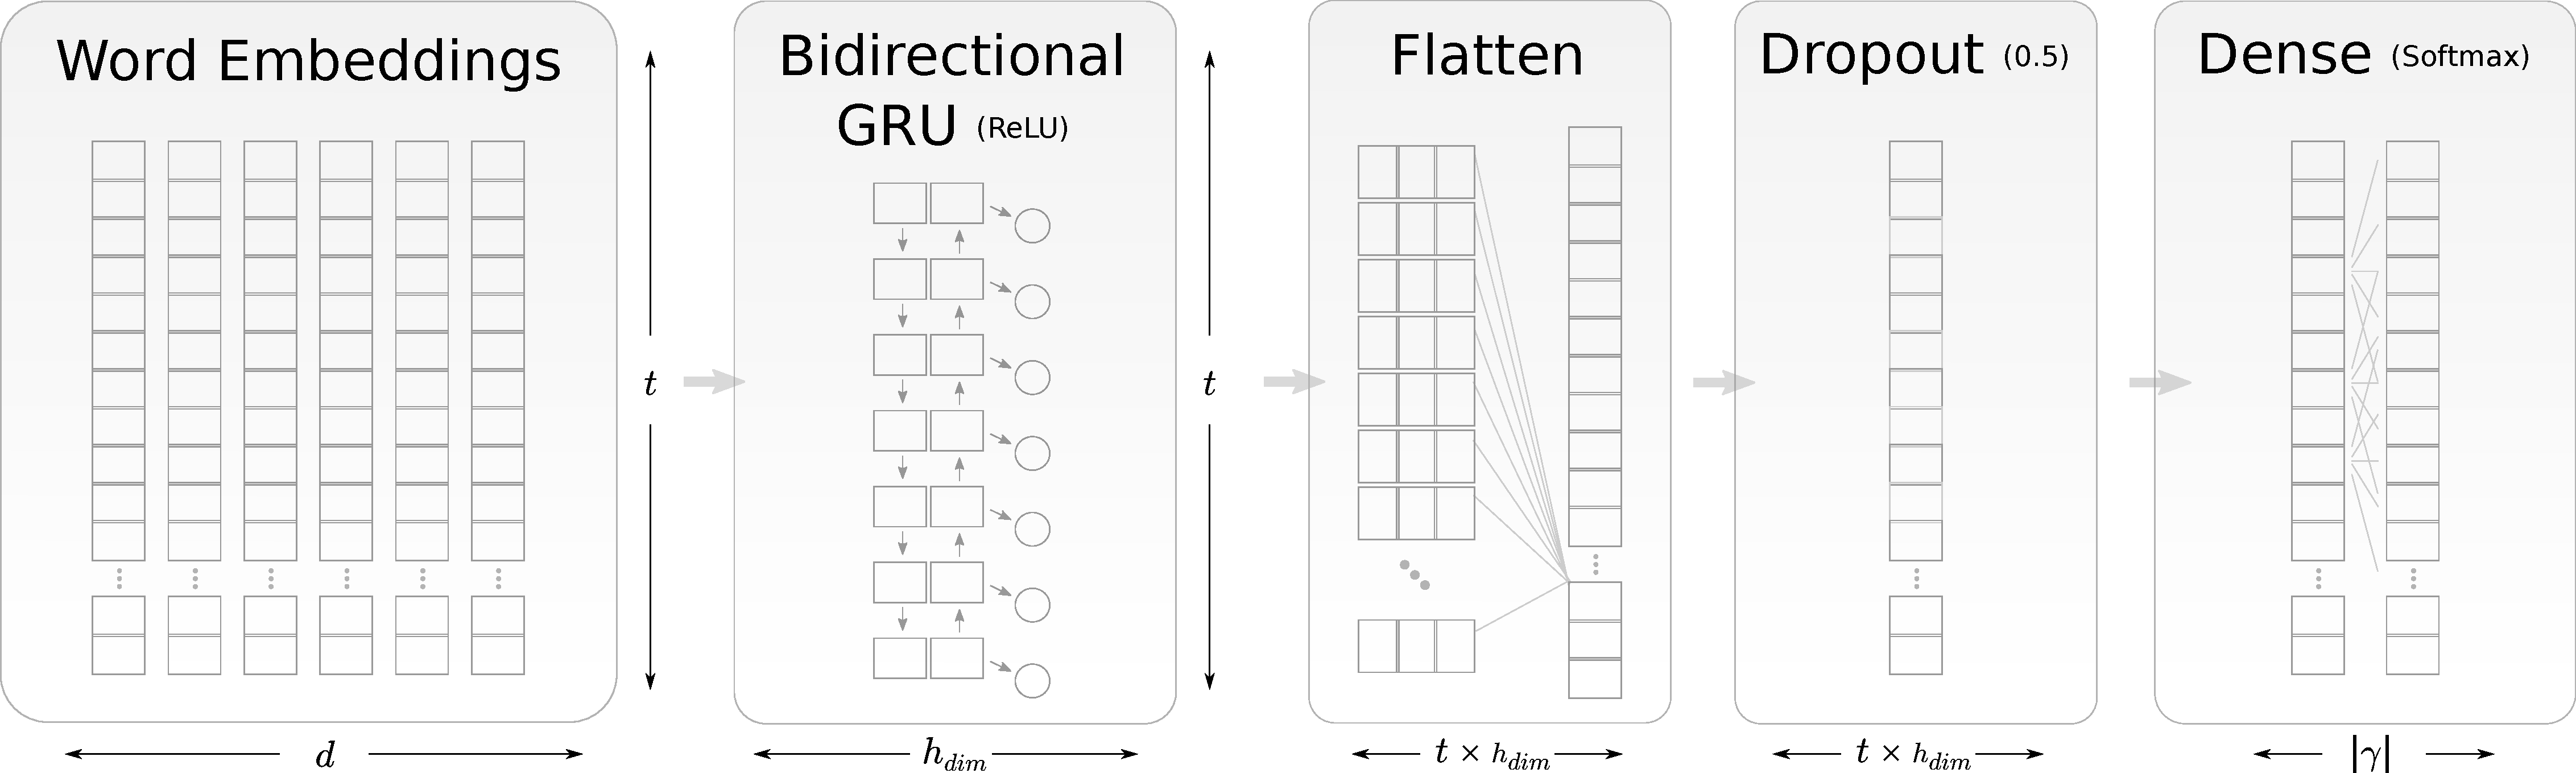
\includegraphics[scale=0.16]{img/recurrent_model_horizontal.pdf}
      \end{center}
  \end{figure}

  \begin{itemize}
    \item GRU: Camada recorrente com memória
    \begin{itemize}
      \item[-] Cada palavra da janela vai possuir uma representação vetorial com tamanho $h_{dim}$
    \end{itemize}
  \end{itemize}

\end{frame}



\begin{frame}[fragile]
\frametitle{Treinamento e Predição}
  
  \begin{itemize}
    \item \textbf{Treinamento:}

    \begin{itemize}
      \item[-] Minimização da função de custo

      \item[\ ] \ 

      \item[-] \textit{Categorical Cross-entropy}: 

      \item[\ ] $J(\theta) = - \frac{1}{m} \sum\limits_{i=1}^{m} \Big[ y_ilog(\hat{y}_i) + (1 - y_i)log(1 - \hat{y}_i) \Big]$

      \item[\ ] \ 

      \item[-] Otimizador: Adadelta
      
    \end{itemize}

    \item[\ ] \ 

    \item \textbf{Predição:}
    \begin{itemize}
      \item[-] Saída da rede neural: $c_{x_i} = \hat{y}_i$
    \end{itemize}

  \end{itemize}

\end{frame}






\begin{frame}
  \frametitle{Roteiro}
  % \setbeamertemplate{section in toc}[mine]
  % \tableofcontents[hideallsubsections]


  \begin{itemize}

  % \vspace{-1em}

    
    \item[\color{gray}{$\bullet$}] \textcolor{gray}{Introdução}
    % \begin{itemize}
    %   \item[\ ] \textit{Part-of-speech} (POS) Tagging 
    %   \item[\ ] O problema
    %   \item[\ ] Objetivos
    % \end{itemize}
    
    
    \item[\color{gray}{$\bullet$}] \textcolor{gray}{Fundamentação}
    % \begin{itemize}
    %   \item[\ ] Aprendizado de máquina
    %   \item[\ ] Córpus
    %   \item[\ ] Representação de palavras
    %   \item[\ ] Redes neurais
    %   \item[\ ] Aprendizagem profunda
    % \end{itemize}


    
    \item[\color{gray}{$\bullet$}] \textcolor{gray}{Trabalhos relacionados}

    
    \item[\color{gray}{$\bullet$}] \textcolor{gray}{Modelo neural recursivo}
    % \begin{itemize}
    %   \item[\ ] Pré-processamento
    %   \item[\ ] Arquitetura
    %   \item[\ ] Treinamento
    %   \item[\ ] Predição
    % \end{itemize}

    
    \item[\color{gray}{$\bullet$}] \textcolor{gray}{Modelo neural recorrente bidirecional}
    % \begin{itemize}
    %   \item[\ ] Pré-processamento
    %   \item[\ ] Arquitetura
    %   \item[\ ] Treinamento e Predição
    % \end{itemize}


    
    \item Testes e resultados
    \begin{itemize}
      \item[\ ] Ambiente de teste
      \item[\ ] Pré-processamento
      \item[\ ] Hiperparâmetros
      \item[\ ] Resultados
      \item[\ ] Comparação com trabalhos relacionados
    \end{itemize}

    \color{gray}
    \item[\color{gray}{$\bullet$}] Considerações finais
    % \begin{itemize}
    %   \item[\ ] Conclusão
    %   \item[\ ] Trabalhos futuros
    % \end{itemize}

  \end{itemize}

\end{frame}











\section{Testes e resultados}

\begin{frame}[fragile]
  \frametitle{Ambiente de teste}

  \begin{itemize}

    \item \textbf{Bibliotecas:}
    \begin{itemize}
      \item[-] Theano: Bib. que otimiza e avalia expressões matemáticas
      \item[-] Keras: Bib. para aprendizagem profunda
      \item[-] Numpy: Bib. para operações com matrizes
      \item[-] gensim: Bib. que possui um \textit{parser} dos \textit{dumps} da Wikipédia
    \end{itemize}

    \item[\ ] \ 

    \item \textbf{Máquina:}
    \begin{itemize}
      \item[-] Sistema operacional: Ubuntu 14.04 LTS
      \item[-] Processador: Intel Xeon X5690 CPU @ 3.47GHz $\times$ 24
      \item[-] Memória: 64GB 1333 MHz DDR3
      \item[-] Python 3.4.3
    \end{itemize}

  \end{itemize}

\end{frame}


\begin{frame}[fragile]
  \frametitle{Pré-processamento}

  \begin{itemize}

    \item Transformação de palavras raras em \texttt{<unknown>}

    \item[\ ] \ 

    \item Transformação de todos os dígitos em ``9''

    \item[\ ] \ 

    \item Utilização de \textit{features} de prefixos, sufixos e capitalização

    \item[\ ] \ 

    \item Utilização de vetores distribuídos de palavras:

    \begin{itemize}
      \item[-] Treinamento não-supervisionado com um \textit{dump} de artigos da Wikipédia: 
      \begin{itemize}
        \item[-] 44 milhões de \textit{tokens}
        \item[-] 618966 vetores
      \end{itemize}
    \end{itemize}
    
    \item[\ ] \ 

    \item Utilização de um vetor aleatório compartilhado para palavras fora do vocabulário

  \end{itemize}

\end{frame}


\begin{frame}[fragile]
  \frametitle{Hiperparâmetros}

  \begin{itemize}

    \item A maioria foi escolhida de modo empírico

    \item Os hiperparâmetros não foram micro-ajustados

  \end{itemize}

  \begin{table}[!htb]
  \scriptsize
  \centering
  \begin{tabular}{lcc}
    \toprule
    \textbf{Hiperparâmetro} & \textbf{Modelo recursivo} & \textbf{Modelo recorrente bidirecional}  \\
    \midrule
    Tamanho da janela de palavras     & 5 & 11 \\
    Tamanho da janela de etiquetas      & 5 & - \\
    Tamanho dos vetores de palavras     & 50 & 50\\
    Tamanho dos vetores de capitalização  & 7 & 7 \\
    Tamanho dos vetores de prefixos     & 5 & 5 \\
    Tamanho dos vetores de sufixos    & 5 & 5 \\
    Número de unidades ocultas      & 250 & 250 \\
    Taxa de \textit{Dropout}      & 0.5 & 0.5 \\
    Taxa de aprendizagem          & 1.0 & 1.0 \\
    Épocas de treinamento         & 3 & 20 \\
    Tamanho do \textit{beam}        & 3 & - \\
    Taxa de raridade            & 5 & 5 \\
    \bottomrule
  \end{tabular}
  \end{table}

\end{frame}




\begin{frame}[fragile]
  \frametitle{Resultados}

  \begin{itemize}

    \item Utilizamos três \textit{córpus} nos experimentos:
    \begin{itemize}
      \item[-] Mac-Morpho original (versão 1)
      \item[-] Mac-Morpho revisado (versão 3)
      \item[-] Tycho Brahe
    \end{itemize}

     \item[\ ] \ 

    \item Dividimos o conjunto de dados em:
    \begin{itemize}
      \item[-] 80\% para treinamento
      \item[-] 20\% para validação
    \end{itemize}

    \item[\ ] \ 

    \item Utilizamos três tipos de vetores distribuídos:
    \begin{itemize}
      \item[-] Word2Vec
      \item[-] Wang2Vec
      \item[-] Fonseca (Treinados por \citeonline{fonseca2015evaluating})
    \end{itemize}

  \end{itemize}

\end{frame}



\begin{frame}[fragile]
  \frametitle{Resultados - Acurácia}

    \begin{equation} \nonumber
      \frac{1}{m} \sum\limits_{i=1}^{m} equal(\hat{y}_i, y_i) 
    \end{equation}

    \begin{itemize}

      \item Para palavras conhecidas

      \item[\ ] \

      \item Para palavras desconhecidas

      \item[\ ] \

      \item Para palavras ambíguas

      \item[\ ] \

      \item Para sentenças

      \begin{itemize}
        \item[-] Sentença é dita correta se todas as palavras na sentença foram classificadas corretamente
      \end{itemize}

    \end{itemize}


\end{frame}


\begin{frame}[fragile]
  \frametitle{Resultados - Modelo neural recursivo}

  \begin{table}[!htb]
  \scriptsize
  \centering
  \begin{tabular}{m{1.5cm}P{1.5cm}P{1.5cm}P{1.5cm}P{1cm}P{1.5cm}}
    \multicolumn{6}{c}{\footnotesize{Acurácia sobre o Mac-Morpho original}} \\
    \toprule
    \textbf{Representação} & \textbf{Conhecidas}  & \textbf{Desconhecidas} & \textbf{Ambíguas} & \textbf{Total} & \textbf{Sentenças} \\
    \midrule
    Word2Vec  & 94.80\% & 82.54\% & 94.24\% & 94.28\% & 46.39\%  \\ % FEITO
    Wang2Vec  & 94.44\% & 82.12\% & 94.53\% & 93.91\% & 46.28\%  \\
    Fonseca   & \textbf{95.92}\% & \textbf{86.77}\% & \textbf{95.26}\% & \textbf{95.53}\% & \textbf{47.39}\%  \\
    \bottomrule
  \end{tabular}
  \end{table}


  \begin{table}[!htb]
  \scriptsize
  \centering
  \begin{tabular}{m{1.5cm}P{1.5cm}P{1.5cm}P{1.5cm}P{1cm}P{1.5cm}}
    \multicolumn{6}{c}{\footnotesize{Acurácia sobre o Mac-Morpho revisado}} \\
    \toprule
    \textbf{Representação} & \textbf{Conhecidas}  & \textbf{Desconhecidas} & \textbf{Ambíguas} & \textbf{Total} & \textbf{Sentenças} \\
    \midrule
    Word2Vec  & 94.13\% & 80.99\% & 93.02\% & 93.78\% & 42.14\% \\ % FEITO (NO SERVIDOR)
    Wang2Vec  & 95.22\% & 81.57\% & 94.17\% & 94.56\% & 42.35\% \\ % FEITO
    Fonseca   & \textbf{96.12\%} & \textbf{88.32\%} & \textbf{96.44\%} & \textbf{95.79\%} & \textbf{47.28\%} \\ % FEITO
    \bottomrule
  \end{tabular}
  \end{table}


  \begin{table}[!htb]
  \scriptsize
  \centering
  \begin{tabular}{m{1.5cm}P{1.5cm}P{1.5cm}P{1.5cm}P{1cm}P{1.5cm}}
    \multicolumn{6}{c}{\footnotesize{Acurácia sobre o Tycho Brahe}} \\
    \toprule
    \textbf{Representação} & \textbf{Conhecidas}  & \textbf{Desconhecidas} & \textbf{Ambíguas} & \textbf{Total} & \textbf{Sentenças} \\
    \midrule
    Word2Vec  & 90.27\% & 48.12\% & 90.81\% & 88.82\% & 22.93\%  \\ % FEITO
    Wang2Vec  & \textbf{91.23}\% & \textbf{48.77}\% & \textbf{90.86}\% & \textbf{89.78}\% & \textbf{23.47}\%  \\ % FEITO
    Fonseca   & 89.74\% & 47.75\% & 89.24\% & 88.31\% & 19.54\%  \\ % FEITO
    \bottomrule
  \end{tabular}
  \end{table}


\end{frame}





\begin{frame}[fragile]
  \frametitle{Resultados - Modelo neural recorrente bidirecional}

  \begin{table}[!htb]
  \scriptsize
  \centering
  \begin{tabular}{m{1.5cm}P{1.5cm}P{1.5cm}P{1.5cm}P{1cm}P{1.5cm}}
    \multicolumn{6}{c}{\footnotesize{Acurácia sobre o Mac-Morpho original}} \\
    \toprule
    \textbf{Representação} & \textbf{Conhecidas}  & \textbf{Desconhecidas} & \textbf{Ambíguas} & \textbf{Total} & \textbf{Sentenças} \\
    \midrule
    Word2Vec  & 97.01\% & 88.79\% & 97.05\% & 97.01\% & 59.43\%  \\ % FEITO
    Wang2Vec  & 97.03\% & 87.60\% & 96.70\% & 96.63\% & 56.63\%  \\ % FEITO
    Fonseca   & \textbf{97.60\%} & \textbf{92.63\%} & \textbf{97.25\%} & \textbf{97.37\%} & \textbf{66.38\%}   \\ % FEITO
    \bottomrule
  \end{tabular}
  \end{table}


  \begin{table}[!htb]
  \scriptsize
  \centering
  \begin{tabular}{m{1.5cm}P{1.5cm}P{1.5cm}P{1.5cm}P{1cm}P{1.5cm}}
    \multicolumn{6}{c}{\footnotesize{Acurácia sobre o Mac-Morpho revisado}} \\
    \toprule
    \textbf{Representação} & \textbf{Conhecidas}  & \textbf{Desconhecidas} & \textbf{Ambíguas} & \textbf{Total} & \textbf{Sentenças} \\
    \midrule
    Word2Vec  & 96.92\% & 87.28\% & 96.30\% & 96.45\% & \textbf{57.03\%} \\ % FEITO
    Wang2Vec  & 97.33\% & 90.03\% & 96.50\% & 96.99\% & 56.04\% \\ % FEITO
    Fonseca   & \textbf{97.33\%} & \textbf{92.18\%} & \textbf{96.50\%} & \textbf{97.08\%} & 56.77\% \\ % FEITO
    \bottomrule
  \end{tabular}
  \end{table}


  \begin{table}[!htb]
  \scriptsize
  \centering
  \begin{tabular}{m{1.5cm}P{1.5cm}P{1.5cm}P{1.5cm}P{1cm}P{1.5cm}}
    \multicolumn{6}{c}{\footnotesize{Acurácia sobre o Tycho Brahe}} \\
    \toprule
    \textbf{Representação} & \textbf{Conhecidas}  & \textbf{Desconhecidas} & \textbf{Ambíguas} & \textbf{Total} & \textbf{Sentenças} \\
    \midrule
    Word2Vec  & 96.42\% & 65.45\% & 95.85\% & 95.53\% & 57.54\%  \\ % FEITO
    Wang2Vec  & 96.33\% & 68.07\% & 95.37\% & 95.36\% & 58.91\%  \\ % FEITO
    Fonseca   & \textbf{96.80\%} & \textbf{73.39\%} & \textbf{96.09\%} & \textbf{96.00\%} & \textbf{64.80\%}  \\ % FEITO
    \bottomrule
  \end{tabular}
  \end{table}


\end{frame}





\begin{frame}[fragile]
  \frametitle{Resultados - Análise}

  \begin{itemize}
    \item Taxa de vetores não encontrados:
  \end{itemize}

  \vspace{-0.25cm}

  \begin{equation} \nonumber
  \frac{\mbox{\footnotesize{\texttt{número de vetores não encontrados}}}}{\mbox{\footnotesize{\texttt{número de palavras no vocabulário}}}}
  \end{equation}

  \vspace{-0.4cm}

  \begin{table}[!htb]
  \scriptsize
  \centering
  \begin{tabular}{lccc}
    \toprule
    \textbf{Representação} & \textbf{Mac-Morpho original (\%)}  & \textbf{Mac-Morpho revisado (\%)} & \textbf{Tycho Brahe (\%)} \\
    \midrule
    Word2Vec  & 33.92 & 27.74 & 78.52 \\ 
    Wang2Vec  & 33.92 & 27.74 & 78.52 \\
    Fonseca   & 39.33 & 32.12 & 93.98 \\
    \bottomrule
  \end{tabular}
  \end{table}

  \ 

  \begin{itemize}
    \item Taxa de ocorrência de vetores não encontrados:
  \end{itemize}

  \vspace{-0.25cm}

  \begin{equation} \nonumber
  \frac{\mbox{\footnotesize{\texttt{ocorrência de vetores não encontrados}}}}{\mbox{\footnotesize{\texttt{número de palavras no conjunto de (treinamento $\cup$ validação)}}}}
  \end{equation}

  \vspace{-0.4cm}

  \begin{table}[!htb]
  \scriptsize
  \centering
  \begin{tabular}{lccc}
    \toprule
    \textbf{Representação} & \textbf{Mac-Morpho original (\%)}  & \textbf{Mac-Morpho revisado (\%)} & \textbf{Tycho Brahe (\%)} \\
    \midrule
    Word2Vec  & 21.01 & 17.11 & 18.42 \\
    Wang2Vec  & 21.01 & 17.11 & 18.42 \\
    Fonseca   & 2.14  & 1.72  & 6.22 \\ 
    \bottomrule
  \end{tabular}
  \end{table}



\end{frame}


\begin{frame}[fragile]
  \frametitle{Comparação com trabalhos relacionados}

  \begin{itemize}
    \item Melhores resultados em cada \textit{córpus}:
  \end{itemize}

  \bgroup
  \renewcommand{\arraystretch}{1.0}
  \hspace*{0cm}\makebox[\linewidth][c]{
  \scriptsize
  \begin{tabular}{m{2cm}cclcclcc}
  \toprule
  \multicolumn{1}{c}{\textbf{\textit{Córpus}}} & \multicolumn{2}{c}{\textbf{Mac-Morpho original}} &  & \multicolumn{2}{c}{\textbf{Mac-Morpho revisado}} &  & \multicolumn{2}{c}{\textbf{Tycho Brahe}} \\ \cline{2-3} \cline{5-6} \cline{8-9} 
  \multicolumn{1}{c}{}               & \textbf{Todas(\%)} & \textbf{FDV(\%)} &  & \textbf{Todas(\%)} & \textbf{FDV(\%)} &  & \textbf{Todas(\%)} &  \textbf{FDV(\%)} \\
  \midrule
  \citeonline{kepler2010variable}    &      -           &    -           &  &  -               &   -             &  &   96,29     &      71,60     \\
  \citeonline{dos2014training}       &     97.47        &   92.49        &  &  -               &   -             &  &   \textbf{97.17}     &      \textbf{86.58}     \\
  \citeonline{fonseca2015evaluating} & \textbf{97.57}   & \textbf{93.38} &  & \textbf{97.33}   &  \textbf{93.66} &  &   96.93     &      84.14     \\
  Este trabalho                      &     97.37        &   92.63        &  &      97.08       &  92.18          &  &   96.00     &      73.39     \\
  \bottomrule
  \end{tabular}
  }
  \egroup

  \begin{itemize}
    \item[\ ] \ 
    \item \textit{dump} da Wikipédia
    \item[\ ] \ 
    \item Modelo de caracteres
  \end{itemize}

\end{frame}







\begin{frame}
  \frametitle{Roteiro}
  % \setbeamertemplate{section in toc}[mine]
  % \tableofcontents[hideallsubsections]


  \begin{itemize}

  % \vspace{-1em}

    
    \item[\color{gray}{$\bullet$}] \textcolor{gray}{Introdução}
    % \begin{itemize}
    %   \item[\ ] \textit{Part-of-speech} (POS) Tagging 
    %   \item[\ ] O problema
    %   \item[\ ] Objetivos
    % \end{itemize}
    
    
    \item[\color{gray}{$\bullet$}] \textcolor{gray}{Fundamentação}
    % \begin{itemize}
    %   \item[\ ] Aprendizado de máquina
    %   \item[\ ] Córpus
    %   \item[\ ] Representação de palavras
    %   \item[\ ] Redes neurais
    %   \item[\ ] Aprendizagem profunda
    % \end{itemize}


    
    \item[\color{gray}{$\bullet$}] \textcolor{gray}{Trabalhos relacionados}

    
    \item[\color{gray}{$\bullet$}] \textcolor{gray}{Modelo neural recursivo}
    % \begin{itemize}
    %   \item[\ ] Pré-processamento
    %   \item[\ ] Arquitetura
    %   \item[\ ] Treinamento
    %   \item[\ ] Predição
    % \end{itemize}

    
    \item[\color{gray}{$\bullet$}] \textcolor{gray}{Modelo neural recorrente bidirecional}
    % \begin{itemize}
    %   \item[\ ] Pré-processamento
    %   \item[\ ] Arquitetura
    %   \item[\ ] Treinamento e Predição
    % \end{itemize}


    
    \item[\color{gray}{$\bullet$}] \textcolor{gray}{Testes e resultados}
    % \begin{itemize}
    %   \item[\ ] Ambiente de teste
    %   \item[\ ] Pré-processamento
    %   \item[\ ] Hiperparâmetros
    %   \item[\ ] Resultados
    %   \item[\ ] Comparação com trabalhos relacionados
    % \end{itemize}

   
    \item Considerações finais
    \begin{itemize}
      \item[\ ] Conclusão
      \item[\ ] Trabalhos futuros
    \end{itemize}

  \end{itemize}

\end{frame}





\begin{frame}[fragile]
  \frametitle{Conclusão}

  \begin{itemize}
    \item Dois modelos para POS Tagging
    \begin{itemize}
      \item Modelo neural recursivo
      \item Modelo neural recorrente bidirecional
    \end{itemize}

    \item[\ ] \ 

    \item Análise de acurácia
    \begin{itemize}
      \item Para três \textit{córpus} diferentes
      \item Para três tipos de vetores distribuídos como representação de palavras
    \end{itemize}

    \item[\ ] \ 

    \item Modelo neural recorrente bidirecional mostrou-se mais eficiente que o recursivo

    \item[\ ] \ 

    \item Segundo melhor resultado para palavras fora do vocabulário no Mac-Morpho original

    \item[\ ] \ 

    \item Criação de uma ferramenta chamada DeepTagger: \url{https://bitbucket.org/fabiokepler/deeptagger}
  \end{itemize}

\end{frame}



\begin{frame}[fragile]
  \frametitle{Trabalhos futuros}

  \begin{itemize}
    \item Realizar mais testes

    \item[\ ] \ 

    \item Revisar o \textit{dump} utilizado: aumentar caso necessário

    \item[\ ] \ 

    \item Melhorar o DeepTagger com novas técnicas:

    \begin{itemize}
      \item Modelo de caracteres

      \item Mecanismos de atenção

      \item Suporte a outras representações distribuídas de vetores
    \end{itemize}
    
    \item[\ ] \ 

    \item Paralelizar o código de treinamento e predição do modelo neural recursivo

  \end{itemize}


\end{frame}



\begin{frame}[fragile]
  \frametitle{Trabalhos futuros}

  \begin{itemize}
    \item Com a inclusão de um modelo de caracteres e trocando GRU por LSTM:
  \end{itemize}

  \bgroup
  \renewcommand{\arraystretch}{1.0}
  \hspace*{0cm}\makebox[\linewidth][c]{
  \scriptsize
  \begin{tabular}{m{2cm}cclcclcc}
  \toprule
  \multicolumn{1}{c}{\textbf{\textit{Córpus}}} & \multicolumn{2}{c}{\textbf{Mac-Morpho original}} &  & \multicolumn{2}{c}{\textbf{Mac-Morpho revisado}} &  & \multicolumn{2}{c}{\textbf{Tycho Brahe}} \\ \cline{2-3} \cline{5-6} \cline{8-9} 
  \multicolumn{1}{c}{}               & \textbf{Todas(\%)} & \textbf{FDV(\%)} &  & \textbf{Todas(\%)} & \textbf{FDV(\%)} &  & \textbf{Todas(\%)} &  \textbf{FDV(\%)} \\
  \midrule
  \citeonline{kepler2010variable}    &      -           &    -           &  &  -               &   -             &  &   96,29     &      71,60     \\
  \citeonline{dos2014training}       &     97.47        &   92.49        &  &  -               &   -             &  &   97.17     &      \textbf{86.58}     \\
  \citeonline{fonseca2015evaluating} & \textbf{97.57}   & \textbf{93.38} &  & \textbf{97.33}   &  \textbf{93.66} &  &   96.93     &      84.14     \\
  Antes                        &     97.37        &   92.63        &  &      97.08       &  92.18          &  &   96.00     &      73.39     \\
  Depois                 &     97.56        &   93.08        &  &      97.29       &  92.84          &  &   \textbf{97.27}     &      84.06     \\
  \bottomrule
  \end{tabular}
  }
  \egroup

  \ 

  \begin{itemize}
  \item Usando os vetores treinados por \citeonline{fonseca2015evaluating}
  \end{itemize}

\end{frame}





\section{Referências}

\begin{frame}[allowframebreaks,noframenumbering]

  \frametitle{Referências}
  \bibliography{bibliografia,abntex2-modelo-references}

\end{frame}



% \plain{Aprendizagem Guiada para Análise Morfossintática usando Redes Neurais Recursivas \\ {\scriptsize asddas}}

% \plain{Aprendizagem Guiada para Análise Morfossintática usando Redes Neurais Recursivas \\ \ \\ {\normalsize asd}}

\plain{Dois modelos de aprendizagem profunda para análise morfossintática \\ \ \\ {\normalsize Marcos Vinícius Treviso} \\ \texttt{\scriptsize marcosvtreviso@gmail.com} \\ \ \\ {\normalsize Orientador: Fabio Natanael Kepler} \\ \ \\ \ \\ {\tiny Trabalho de Conclusão de Curso II} \\ {\normalsize 3 de dezembro de 2015} \\ {\scriptsize Universidade Federal do Pampa}}






\begin{frame}[fragile]
  \frametitle{Aprendizagem profunda}

  \begin{columns}[onlytextwidth]
    \column{0.45\textwidth}
      
      \begin{itemize}
        \item Muitas tranformações não lineares
        \item[\ ] \ 
        \item Objetivo de aprender automaticamente boas \textit{features}
        \item[\ ] \ 
        \item Crescimento do desempenho computacional e criação de novos algoritmos
        \item[\ ] \ 
        \item Redes neurais com múltiplas camadas
      \end{itemize}

    \column{0.55\textwidth}
      
      \begin{figure}
      \begin{center}
        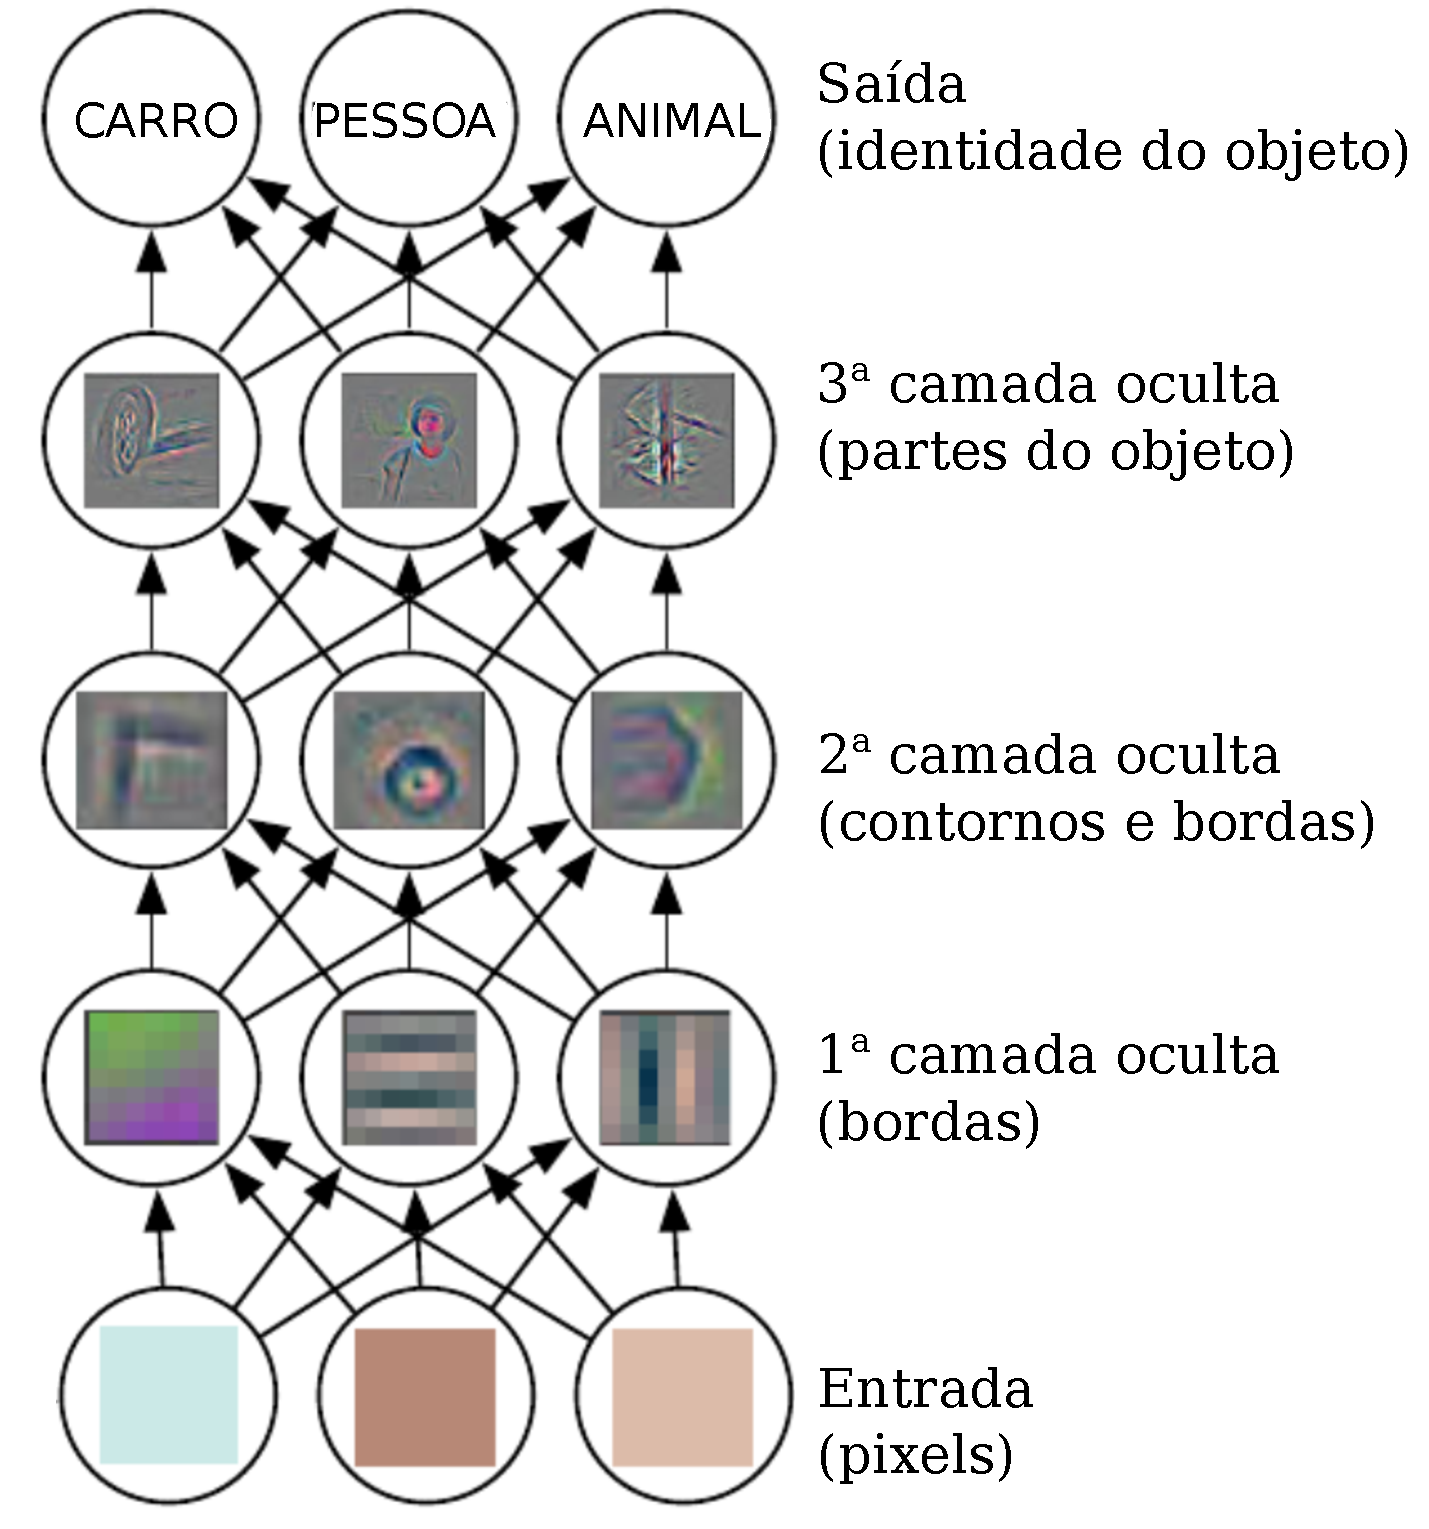
\includegraphics[scale=0.2]{img/aprendendodeep2.pdf}
      \end{center}
      \caption{Adaptado de: \citeonline{Bengio-et-al-2015-Book}}
    \end{figure}
       

  \end{columns}
  

\end{frame}




\begin{frame}[fragile]
  \frametitle{Redes neurais recursivas}

  \begin{itemize}
    \item Grafo computacional parece como uma árvore
  
    \item Aplica-se transformações recursivamente

     % ``Dado um grafo acíclico dirigido, é visitado os nodos em ordem topológica, e recursivamente aplica-se transformações para gerar novas representações a partir de prévias representações já computadas dos nodos filhos''  


    \item Composição da saída com entrada

    \item[\ ] \ 

    \begin{figure}
      \begin{center}
        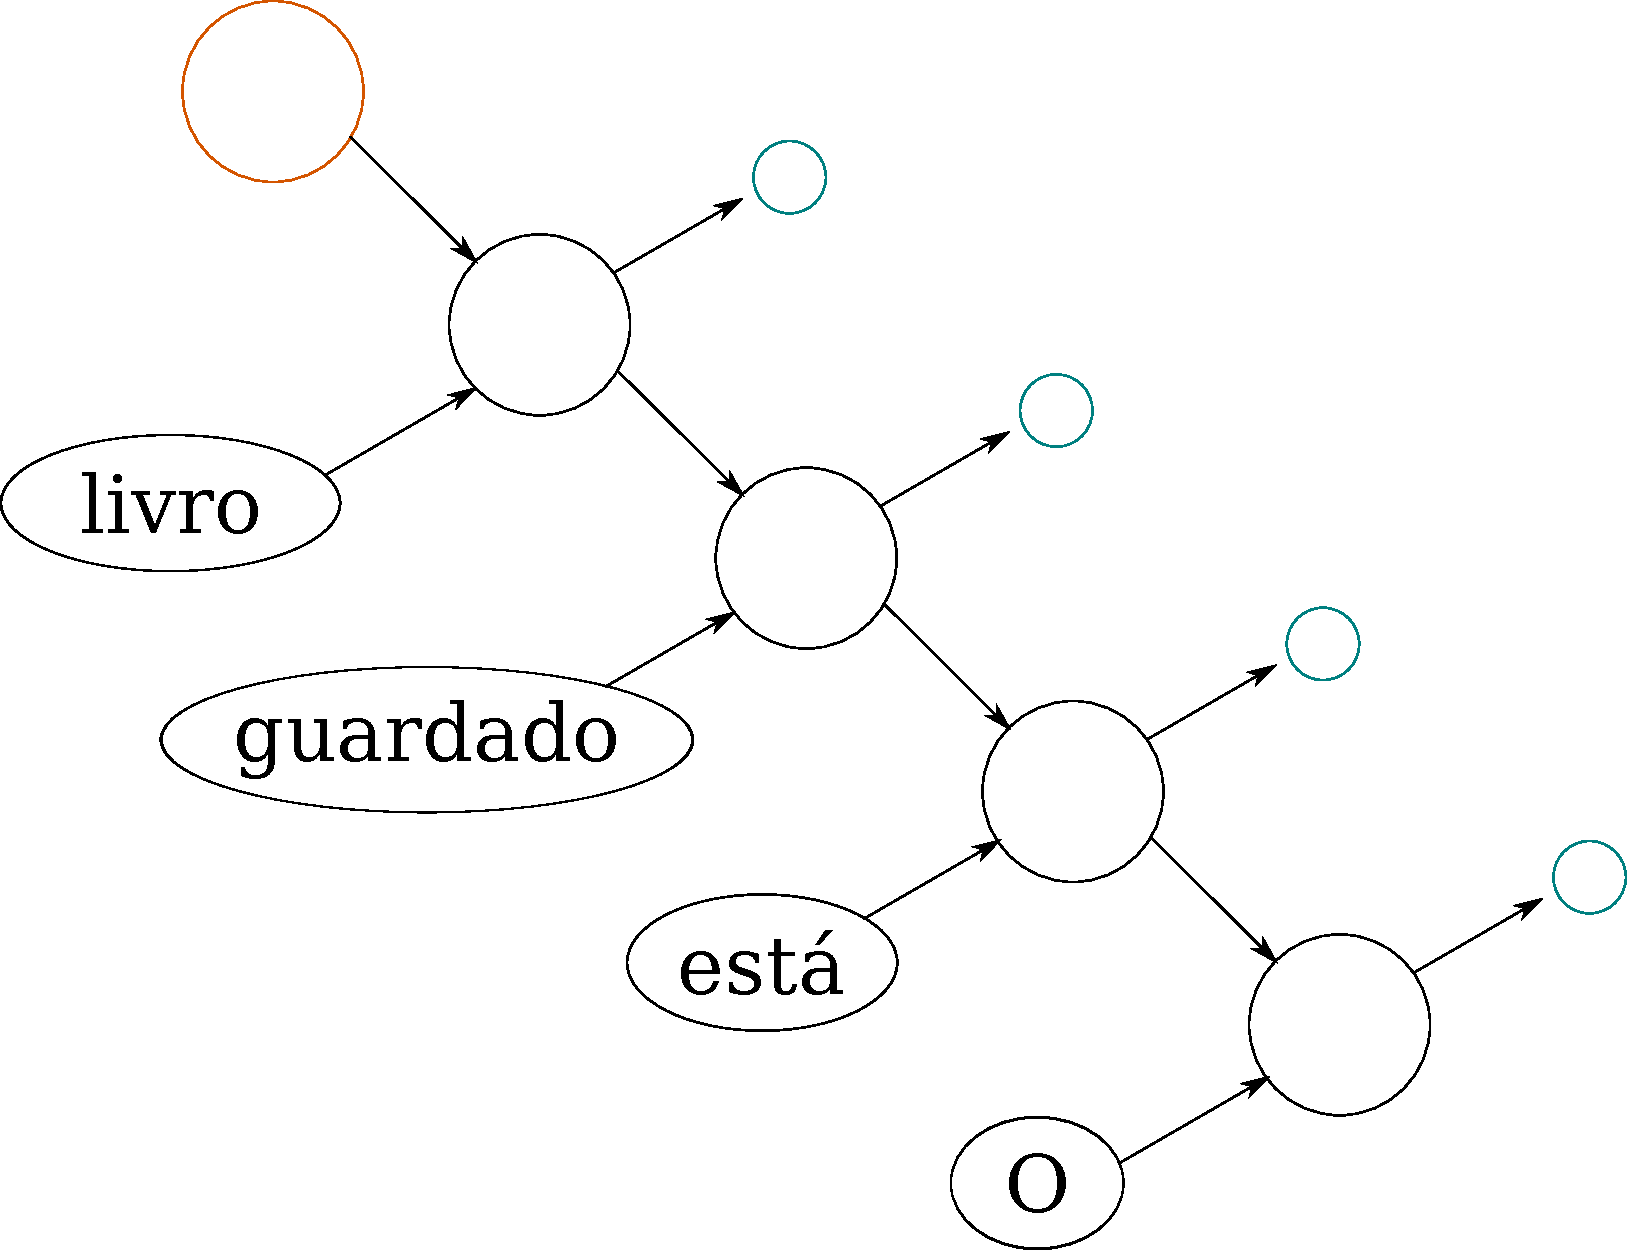
\includegraphics[scale=0.25]{img/redeneuralrecursiva.pdf}
      \end{center}
    \end{figure}


  \end{itemize}

\end{frame}





\end{document}
